% \documentclass[14pt,a4paper]{report}
\documentclass[14pt,a4paper]{article}
\usepackage[utf8]{inputenc}
\usepackage[english,vietnamese]{babel}
\usepackage[left=3.50cm, right=2.00cm, top=2.00cm, bottom=2.00cm]{geometry}
\usepackage{multirow}
\usepackage{listings}
\lstset{basicstyle=\ttfamily,escapechar=\@}
\usepackage{paralist}
\usepackage{graphicx}
\usepackage{wrapfig}
\usepackage{setspace}
\usepackage{amsthm}
\usepackage{array}
\usepackage{hyperref}
\hypersetup{colorlinks=true,pdfencoding=auto}
\usepackage{hypcap}
\usepackage{longtable}
\usepackage{rotating}
\usepackage{subfig}
\usepackage{float}
\renewcommand{\baselinestretch}{1.3}
\usepackage{indentfirst}
\usepackage{pgfgantt}
\usepackage{amsmath}
\usepackage{fancybox}
\usepackage{tabto}
\setcounter{tocdepth}{4}
\setcounter{secnumdepth}{4}
\selectlanguage{vietnamese}

\begin{document}

\newgeometry{top=2cm, bottom=2cm, left=2cm, right=2cm}
\begin{titlepage}
\vspace*{1\bigskipamount}
\begin{otherlanguage*}{vietnamese}
\thispagestyle{empty}
\thisfancypage{
\setlength{\fboxsep}{5pt}
\fbox}{}

\begin{center}
\makeatletter
\fontsize{12}{12}\textbf{ĐẠI HỌC QUỐC GIA TP HỒ CHÍ MINH}\\
\fontsize{14}{14}\textbf{TRƯỜNG ĐẠI HỌC BÁCH KHOA}\\
\fontsize{14}{14} -----------------------------------
\makeatother

\vspace{4cm}

{\makeatletter
\fontsize{16}{16}\textbf{TRẦN HOÀNG TUẤN}\\
\makeatother}

\vspace{4cm}

{\makeatletter
\fontsize{18}{18}\textbf{SINH BIỂU CẢM KHUÔN MẶT DỰA TRÊN PHÙ HỢP GIỌNG NÓI}\\
\makeatother}
\end{center}

{\makeatletter
\begin{flushleft}
\hspace{2cm}\fontsize{14}{14}\textbf{Chuyên ngành: Khoa học dữ liệu}\\
\hspace{2cm}\fontsize{14}{14}\textbf{Mã số: ...}\\
\end{flushleft}
\makeatother}

\begin{center}
\vspace{1.2cm}
{\makeatletter
\fontsize{18}{18}\textbf{LUẬN VĂN THẠC SĨ}\\
\makeatother}


\vspace{8cm}
{\makeatletter
\fontsize{12}{12} TP. HỒ CHÍ MINH - tháng 7, năm 2020\\
\makeatother}
\end{center}

\end{otherlanguage*}
\end{titlepage}


\restoregeometry

\begin{titlepage}

\begin{center}

\vspace*{3\bigskipamount}

\begin{otherlanguage*}{vietnamese}

\makeatletter
\fontsize{12}{12}\textbf{ĐẠI HỌC QUỐC GIA TP HỒ CHÍ MINH}
\makeatother

\makeatletter
\fontsize{14}{14}\textbf{TRƯỜNG ĐẠI HỌC BÁCH KHOA}\\
\fontsize{14}{14} -----------------------------------
\makeatother

\begin{figure}[h]
	\centering
    \includegraphics[width=0.4\columnwidth]{./cover/bk.png}
\end{figure}

{\makeatletter
\fontsize{16}{16}\textbf{TRẦN HOÀNG TUẤN}
\makeatother}

\vspace{1cm}

{\makeatletter
\fontsize{16}{16}\textbf{SINH BIỂU CẢM KHUÔN MẶT DỰA TRÊN PHÙ HỢP GIỌNG NÓI}\\
\vspace{1cm}
\fontsize{12}{12} NGÀNH: KHOA HỌC MÁY TÍNH\\
\fontsize{12}{12} MÃ NGÀNH: 8480101\\
\makeatother}

\vspace{1cm}
{\makeatletter
\fontsize{12}{12}\textbf{LUẬN VĂN THẠC SĨ}\\
\makeatother}

\vspace{1cm}
{\makeatletter
\fontsize{12}{12}\textbf{NGƯỜI HƯỚNG DẪN KHOA HỌC}\\
\fontsize{12}{12}\textbf{TS: NGUYỄN QUANG HÙNG}\\
\makeatother}

\vspace{4cm}
{\makeatletter
\fontsize{12}{12} HỒ CHÍ MINH - 2021\\
\makeatother}

\end{otherlanguage*}

\vfill
\end{center}
\end{titlepage}


\begin{titlepage}
\begin{otherlanguage*}{vietnamese}

    \begin{minipage}[t]{0.42\textwidth}
        \begin{center}
            \fontsize{11.5}{11.5}ĐẠI HỌC QUỐC GIA TPHCM\\
            \textbf{TRƯỜNG ĐẠI HỌC BÁCH KHOA}\\
            \textbf{---------------------------}\\
        \end{center}
    \end{minipage}
    \noindent
    \begin{minipage}[t]{0.57\textwidth}
        \begin{center}
            \fontsize{11.5}{11.5}\textbf{CỘNG HÒA XÃ HỘI CHỦ NGHĨA VIỆT NAM}\\
            \textbf{Độc lập - Tự do - Hạnh phúc}\\
            \textbf{---------------------------}\\
        \end{center}
    \end{minipage}

    \begin{center}
        \fontsize{18}{18}\textbf{NHIỆM VỤ LUẬN VĂN THẠC SĨ}
    \end{center}

    \begin{flushleft}
        Họ tên học viên: Trần Hoàng Tuấn
        \tabto{10cm}
        MSHV: 1970220\\
        Ngày, tháng, năm sinh: 01/08/1996
        \tabto{10cm}
        Nơi sinh: Đồng Nai\\
        Chuyên ngành: Khoa học dữ liệu
        \tabto{10cm}
        Mã số:\\

        \renewcommand{\labelenumi}{\Roman{enumi}}
        \begin{enumerate}
            \item \textbf{TÊN ĐỀ TÀI: SINH BIỂU CẢM KHUÔN MẶT DỰA TRÊN PHÙ HỢP GIỌNG NÓI}
            \item \textbf{NHIỆM VỤ VÀ NỘI DUNG:}
            \item \textbf{NGÀY GIAO NHIỆM VỤ:}
            \item \textbf{NGÀY HOÀN THÀNH NHIỆM VỤ:}
            \item \textbf{CÁN BỘ HƯỚNG DẪN:}
        \end{enumerate}
    \end{flushleft}

    \begin{flushright}
        \textit{Tp.HCM, ngày .... tháng .... năm 2021}
    \end{flushright}

    \begin{center}
        \begin{minipage}[t]{0.40\textwidth}
            \center\textbf{CÁN BỘ HƯỚNG DẪN}\\
            (Họ tên và chữ ký)
            \vspace{3cm}
        \end{minipage}
        \noindent
        \begin{minipage}[t]{0.50\textwidth}
            \center\textbf{CHỦ NHIỆM BỘ MÔN ĐÀO TẠO}\\
            (Họ tên và chữ ký)
            \vspace{3cm}
        \end{minipage}
        \begin{minipage}[t]{0.90\textwidth}
            \center\textbf{TRƯỞNG KHOA}\\
            (Họ tên và chữ ký)
            \vspace{3cm}
        \end{minipage}
    \end{center}

\end{otherlanguage*}
\vfill
\end{titlepage}


\thispagestyle{plain}
\chapter*{\centering \begin{huge}Lời cảm ơn\end{huge}}

\noindent
%\large

Trước hết, tôi xin được bày tỏ sự trân trọng và biết ơn sự giúp đỡ của các thầy hướng dẫn khoa học của tôi, là Tiến sĩ Lê Thành Sách và Tiến sĩ Nguyễn Quang Hùng. Cảm ơn các thầy vì đã góp ý, giúp đỡ về mặt khoa học và kiến thức trong suốt thời gian thực hiện đề tài. Tôi cũng chân thành gửi lời cảm ơn tới quý thầy cô tại Trường Đại học Bách Khoa TPHCM, những người đã giúp đỡ và cung cấp cho tôi những kiến thức khoa học để tôi có thể vững bước phát triển sự nghiệp trong tương lai.

Tôi xin được gửi lời cảm ơn đặc biệt và sâu sắc đến gia đình và những người bạn của tôi, những người đã kề vai sát cánh, giúp đỡ, động viên và dành những điều kiện tốt nhất để cho tôi được học tập trong suốt những năm vừa qua.

Luận văn chắc chắn không thể tránh khỏi những hạn chế và thiếu sót, nên tôi hy vọng sẽ nhận được nhiều lời góp ý quý báu cũng như những ý tưởng mới từ quý thầy cô hội đồng và các bạn đọc để đề tài ngày càng hoàn thiện hơn. Một lần nữa, tôi xin chân thành cảm ơn.

\begin{flushright}
    Hồ Chí Minh, ngày 05 tháng 08 năm 2021


    Trần Hoàng Tuấn
    \end{flushright}

\clearpage

\thispagestyle{plain}
\chapter*{\centering \begin{huge}Abstract\end{huge}}

\noindent
%\large
\textit{Speech-driven facial animation} is a hot research topic in recent years since it has many applications in our real life. The aim of this problem is to generate videos that synthesize a talking face of an arbitrary person based on speech audio. It also comes with many challenges. The synthesized videos are considered high quality when the shape of mouth has high correlation with the given speech, the human face in video should be created as real as possible and identity of the person should be kept. This research proposes a method to generate facial animation from speech. Our approach inherits from this paper \cite{chen2019}, we also use the facial landmark normalization method from the paper \cite{gen_face_landmark} to improve video quality. In the paper \cite{chen2019}, they design a cascade deep learning system to effectively synthesize talking face video. This method uses a neural network to convert speech audio to a facial landmark sequence that describes face movement. In the end, they use a GANs network to generate video based on the landmark sequence that has just been created in the last step. At the step of creating a landmark sequence, we apply the normalization method from \cite{gen_face_landmark} with some modification so that it can be fitted to our system. It helps our system to create more realistic and high quality videos. All experiments in this thesis are performed on these two datasets: GRID \cite{grid} and LRW \cite{lrw}. The result shows that our approach creates videos with higher quality than the baseline method.

\clearpage
\begin{titlepage}
\begin{otherlanguage*}{vietnamese}

\begin{center}
    \fontsize{18}{18}\textbf{LỜI CAM ĐOAN}
\end{center}

Tôi xin cam đoan luận văn \textbf{"SINH BIỂU CẢM KHUÔN MẶT DỰA TRÊN PHÙ HỢP GIỌNG NÓI"} là công trình nghiên cứu của riêng tôi.
\par
Các số liệu trong luận văn được sử dụng trung thực, kết quả nghiên cứu trong luận văn này chưa từng được công bô tại bất kì công trình nào khác.

\begin{flushright}
    \begin{minipage}[t]{0.40\textwidth}
    \begin{center}
        TPHCM, ngày .... tháng .... năm 2021\\
        Tác giả luận văn\\
        \vspace{3cm}
        \textbf{Trần Hoàng Tuấn}
    \end{center}
    \end{minipage}
\end{flushright}


\end{otherlanguage*}
\vfill
\end{titlepage}

\pagenumbering{gobble}
\tableofcontents
\listoffigures

\pagenumbering{arabic}

\section{\texorpdfstring{Tóm tắt luận văn}{brief}}
% Trình bày ngắn gọn về cấu trúc của Luận văn, giới thiệu những điểm nhấn của Luận văn, kết quả, và các từ khóa đi kèm.

\include{./content/open}
\section{\texorpdfstring{Tổng quan tình hình nghiên cứu}{overview}}
% Sơ lược, phân tích, đánh giá các công trình nghiên cứu nổi tiếng có liên quan đến đề tài. Nêu những vấn đề bức thiết cần phải giải quyết, chỉ ra những thiếu sót mà những nghiên cứu trước đây chưa giải quyết được.
Để tạo sinh mặt người đang nói, các công trình nghiên cứu tập trung chủ yếu vào vùng miệng. Bài nghiên cứu vào năm 2018 của Lele Chen \cite{chen2018} đưa ra phương pháp tạo sinh video vùng miệng của người đang nói với đầu vào là ảnh tĩnh của khuôn miệng và một đoạn âm thanh có chứa tiếng nói. Vào năm 2019, Lele Chen \cite{chen2019} và Vougioukas \cite{vougioukas2019} tiếp tục đưa ra phương pháp tạo sinh cả khuôn mặt người dựa vào ảnh tĩnh của khuôn mặt và đoạn âm thanh chứa tiếng nói. Năm 2020, Vougioukas \cite{vougioukas2020} đã cải tiến phương pháp tạo sinh mặt và cập nhật thêm hành động chớp mắt, Lele Chen \cite{chen2020} cũng đưa ra phương pháp mới để tạo sinh mặt hiệu quả hơn, tự nhiên hơn với việc di chuyển của vùng đầu trên khung hình.

Nhìn chung, các nghiên cứu này đã đưa ra các kiến trúc mạng hiệu quả để tạo sinh khuôn mặt cũng như các phương pháp, lập luận và chứng minh tính hiệu quả của các kiến trúc mạng được đề xuất. Mặc dù các thông số của thử nghiệm đưa ra là khá tốt, các nghiên cứu của Vougioukas vẫn chưa thể tạo ra chuyển động của đầu, kết quả tạo sinh của Vougioukas đôi khi không giữ được đặc trưng của ảnh. Nghiên cứu của Lele Chen năm 2020 \cite{chen2020} đã tạo ra chuyển động cho phần đầu dựa trên tiếng nói, nhưng khuôn mặt được tạo sinh vẫn còn có thể bị nhận ra qua các phép thử Turing, và chuyển động của đầu đôi khi vẫn chưa được tự nhiên, mạng cũng có cấu trúc rất phức tạp và đòi hỏi nhiều tài nguyên tính toán để có thể huấn luyện.

\section{\texorpdfstring{Mục tiêu và nhiệm vụ nghiên cứu}{target_and_mission}}
%Mục tiêu và nhiệm vụ nghiên cứu

\subsection{\texorpdfstring{Mục tiêu}{Target}}
Mục tiêu của Luận văn Tốt nghiệp là nghiên cứu các đề tài có liên quan bằng cách khảo sát, kiểm định và thử nghiệm các nghiên cứu mới nhất hiện có, qua đó tiến hành các thử nghiệm để đưa ra một mô hình tạo sinh mặt người đang nói có độ chính xác cao và chân thật. Hình ảnh được tạo ra phải sắc nét, ít nhiễu và tương đồng về mặt nhận dạng, cấu trúc với hình ảnh người mẫu. Đồng thời, khẩu hình miệng của hình ảnh được tạo ra phải khớp với tiếng nói, phù hợp với cách phát âm từ ngữ. Bên cạnh đó, video được tạo ra phải có tính liền lạc, ổn định, không bị hiện tượng nhảy hình. Mục tiêu được đặt ra nhằm thử nghiệm các mô hình hiện có, tăng tính ứng dụng của việc tạo sinh mặt người vào thực tiễn cuộc sống.

\section{\texorpdfstring{Cơ sở lý thuyết}{base_knowledge}}
%Trình bày cơ sở lý thuyết, các lập luận, căn cứ khoa học được sử dụng trong Luận văn.

\subsection{\texorpdfstring{Trí tuệ nhân tạo, học máy và học sâu}{ai_ml_dl}}

Định nghĩa:
\begin{itemize}
    \item \textbf{Trí tuệ nhân tạo:} Là ngành nghiên cứu về cách thực hiện các chương trình máy tính có khả năng mô phỏng suy nghĩ và khả năng giải quyết vấn đề ở cấp độ con người
    \item \textbf{Học máy:} Là tập con của ngành trí tuệ nhân tạo, là ngành nghiên cứu cách thực hiện các chương trình máy tính mà không phải có mã lập trình tường minh, có chức năng tự động học các tri thức của con người để cải thiện các quyết định của nó trên các dữ liệu mà nó chưa từng gặp trước đây.
    \item \textbf{Học sâu:} Là tập con của ngành học máy, là tập hợp các giải thuật học máy có sử dụng mạng thần kinh nhân tạo có cấu trúc tương tự mạng thần kinh trong não bộ con người để học cách đưa ra quyết định.
\end{itemize}

\begin{figure}[H]
    \centering
    \includegraphics[width=7cm]{./content/materials/ai_ml_dl.png}
    \caption{Trí tuệ nhân tạo, học máy và học sâu}
\end{figure}


Ngày nay, ngành học máy và học sâu ngày càng chiếm nhiều ưu thế so với các phương pháp khác trong các ứng dụng thực tế do có độ tổng quát dữ liệu tốt, độ chính xác cao, và có thể mô hình hóa các vấn đề phức tạp, trừu tượng trong đời sống. Đối với các vấn đề phức tạp như thị giác máy, dịch máy, đánh nhãn văn bản tự động, tạo sinh dữ liệu,... các giải thuật học sâu luôn là lựa chọn hoàn hảo do nó có khả năng tổng quát hóa một lượng dữ liệu rất lớn. Một lợi điểm khác của việc sử dụng các giải thuật học sâu là các giải thuật này có khả năng tìm ra các đặc trưng của dữ liệu một cách tự động. Trong khi các giải thuật học máy truyền thống chỉ có khả năng xử lý tốt trên dữ liệu đã được rút trích đặc trưng bằng các giải thuật xử lý dữ liệu truyền thống, các mạng học sâu có khả năng tự học lấy các đặc trưng của dữ liệu. Tuy nhiên, các giải thuật học sâu yêu cầu một lượng dữ liệu lớn để học. Bên cạnh đó, bài toán phải được mô hình hóa hợp lý, mạng thần kinh học sâu cũng phải được thiết kế phù hợp với mô hình bài toán để khiến cho việc học của mạng thần kinh dễ dàng và hiệu quả hơn.

\subsection{\texorpdfstring{Tính chất tổng quát hóa dữ liệu của mạng thần kinh học sâu}{dl_network}}
Mạng thần kinh học sâu có khả năng tổng quát hóa dữ liệu cao, nhờ vào đó, nó có thể được huấn luyện để học bất cứ thứ gì nếu nó được mô hình hóa một cách hợp lý. Một mạng học sâu đạt được mức độ tổng quát hóa dữ liệu cao bằng cách học những đặc trưng ẩn của dữ liệu được dùng để huấn luyện nó. Vì vậy, mạng học sâu có thể đưa ra dự đoán trên những dữ liệu mới mà nó chưa từng nhìn thấy nhờ vào việc nội suy, nhưng những dữ liệu đó phải tương tự với dữ liệu được dùng để huấn luyện nó. Với những dữ liệu nằm ngoài phân phối dữ liệu huấn luyện, mạng thần kinh học sâu sẽ không có khả năng đưa ra kết quả chính xác bởi cấu trúc và các thông số trong mạng thần kinh không được điều chỉnh đề phù hợp với những dữ liệu đó.

\subsection{\texorpdfstring{Các cấu trúc trong mạng học sâu được sử dụng trong luận văn}{dl_basic_structures}}

\subsubsection{Mạng thần kinh tích chập (Convolution)}
Trước khi có mạng học sâu, việc trích xuất đặc trưng bằng các kĩ thuật đặc biệt cho từng loại dữ liệu khác nhau là công đoạn quan trọng nhất trong quá trình giải quyết một bài toán. Lý do là bởi mạng thần kinh truyền thống không có khả năng tạo ra các chiều không gian đủ rộng để tự học các đặc trưng của dữ liệu. Thông thường, phép tích chập được thực hiện bằng các nhân tích chập (kernel). Một phép tích chập được đặc trưng bởi số lượng kênh đầu vào, số lượng kênh đầu ra và kích thước của nhân tích chập.

\begin{figure}[H]
    \centering
    \includegraphics[width=15cm]{./content/materials/cnn.png}
    \caption{Cách tính tích chập. Nguồn: Internet}
\end{figure}

Ví dụ, một phép tích chập với nhân có kích thước $m$x$m$ được thực hiện trên một ma trận ba chiều kích thước $H$x$H$x$K$ sẽ cho ta một ma trận kết quả có kích thước $(N-m+1)$x$(N-m+1)$
Phép tích chập cho ma trận hai chiều trong mạng được biểu diễn bởi phương trình sau:

\begin{equation}
    o_{ijm}=\sum_{k=0}^{K-1}\sum_{p=0}^{H-1}\sum_{q=0}^{H-1}x_{i+p,j+q,k}^{(l-1)}w_{pqkm}+b_{ijm}
\end{equation}

Sự xuất hiện của mạng thần kinh tích chập đã giúp cho việc trích xuất đặc trưng trở nên dễ dàng hơn và đôi khi là không cần thiết nhờ vào khả năng tự động trích xuất đặc trưng của mạng. Sở dĩ mạng thần kinh tích chập có khả năng trích xuất đặc trưng tốt là nhờ vào việc nó tập trung vào học các kiễu mẫu rất chi tiết hay xuất hiện trong dữ liệu ở các lớp đầu. Ở các lớp sau, những tri thức học được càng được tổng quát dần bằng việc kết hợp các tri thức học được từ lớp trước vào tạo nên những hiểu biết ở bậc cao nhất của dữ liệu ở các lớp tích chập cuối cùng.

Nhưng điều này không có nghĩa là chỉ cần sử dụng mạng thần kinh tích chập thì ta sẽ không cần quan tâm tới việc trích xuất đặc trưng nữa bởi khi có những đặc trưng tốt được đưa vào mạng, mạng tích chập vẫn cho ra kết quả tốt hơn, chính xác hơn với ít dữ liệu hơn và thời gian huấn luyện cũng nhanh hơn. Ngoài ra, lớp tích chập cũng có số lượng hệ số học nhỏ, huấn luyện nhanh, vì vậy nó hay được đặt nằm ở các lớp đầu và giữa trong các mạng học sâu để trích xuất dữ liệu nhanh và hiệu quả hơn.

\subsubsection{Tích chập ngược (Deconvolution)}

Đây là mạng có tính năng ngược với mạng tích chập đã được nêu ở phần trên. Nếu như mạng tích chập có chức năng mã hóa, rút trích đặc trưng của dữ liệu đầu vào, thì mạng tích chập ngược nhận vào những đặc trưng đã được rút trích của dữ liệu và tạo sinh ngược lại dữ liệu với cấu trức tương tự ban đầu. Phép tích chập ngược cũng được đặc trưng bởi kích thước nhân, số lượng kênh đầu vào và đầu ra.

Phép tích chập ngược thường hay được sử dụng để tái thiết lập lại cấu trúc ban đầu. Thay vì rút trích và thu nhỏ dữ liệu ban đầu thành những đặc trưng như mạng tích chập, mạng tích chập ngược sử dụng các đặc trưng đã được rút trích và học các trọng số để tạo ra dữ liệu mới có cấu trúc giống với dữ liệu được trích xuất đặc trưng ban đầu. Vì vậy, mạng tích chập ngược có tính năng tạo sin dữ liệu và hay được sử dụng trong các ứng dụng như:

\begin{itemize}
    \item \textbf{Autoencoder:} Một mạng tích chập thu nhỏ và rút trích đặc trưng từ dữ liệu gốc, mạng tích chập ngược dùng véc tơ đặc trưng để cố gắng tái tạo lại dữ liệu gốc.
    \item \textbf{Bài toán phân đoạn ảnh:} Đánh nhãn cho từng điểm ảnh để xem nó thuộc vào lớp nào. Sau khi rút trích đặc trưng từ ảnh, mạng tích chập ngược được dùng để biên dịch đặc trưng ảnh thành mặt nạ phân lớp cho ảnh.
    \item \textbf{Variational Autoencoder:} Một loại mạng nơ ron dùng để tạo sinh dữ liệu dựa trên phân phối xác suất mà nó học được từ dữ liệu mẫu. Với phân phối xác suất học được, mạng có thể tạo ra được dữ liệu có tính chất, cấu trúc tương tự như dữ liệu mẫu nhưng chưa từng tồn tại trong dữ liệu mẫu. Ví dụ: cho mạng Variational Autoencoder học cách tạo sinh hình ảnh của các chữ số trong tập MNIST, sau đây là ảnh được tạo sinh: 
        \begin{figure}[H]
            \centering
            \includegraphics[width=7cm]{./content/materials/mnist_vae.png}
            \caption{Tạo sinh ảnh cùng phân phối xác suất với tập dữ liệu MNIST}
        \end{figure}
    \item \textbf{Mạng GANs (Generative Adversarial Networks):} Là một loại mạng tạo sinh dữ liệu bằng cách học cấu trúc dữ liệu của các mẫu được dùng để huấn luyện, và cũng là cấu trúc mạng được dùng trong luận văn.
\end{itemize}

\subsubsection{Lớp kết nối đầy đủ (Fully Connected)}
Lớp kết nối đầy đủ là lớp chính của mạng nơ ron truyền thống và được xem là một phép biến đổi tuyến tính trong mạng học sâu với phương trình:
\begin{equation}
    y=xA^T+b
\end{equation}
Với phương trình trên, lớp kết nối đầy đủ là một mạng lưới perceptron đơn lớp, với:
\begin{itemize}
    \item Đầu vào là véc tơ $x$ với $N_x$ chiều
    \item Đầu ra là véc tơ $y$ với $N_y$ chiều
    \item Véc tơ $b$ có $N_y$ chiều
    \item $A$ là ma trận có kích thước $N_y$x$N_x$
\end{itemize}
Trong mạng học sâu, lớp kết nối đầy đủ thường được đặt ở vị trí sâu nhất của mạng để thực hiện biến đổi tuyến tính cuối cùng từ những đặc trưng được trích xuất từ các lớp trước đó để cho ra kết quả cuối cùng nhờ vào khả năng học những đặc trưng tổng quát. Tuy nhiên, đây không phải là lớp biến đổi dữ liệu có khả năng học được các đặc trưng dữ liệu ở mức độ chi tiết như mạng tích chập, có số lượng trọng số học lớn và chỉ đặc trưng duy nhất cho một bài toán, không thể tái sử dụng lại cho bài toán khác.

\subsubsection{Mạng nơ ron hồi quy (RNN)}

Trong cuộc sống hằng ngày, đôi khi ta phải xử lý các loại dữ liệu có tính chất chuỗi, đó là các dữ liệu có tính trật tự. Khác với kiểu dữ liệu truyền thống khi mà các mẫu dữ liệu không có tính chất chuỗi, không có thứ tự và độc lập lẫn nhau, đối với dữ liệu chuỗi, thứ tự của các mẫu dữ liệu là quan trọng và mang ý nghĩa nhất định. Nếu thứ tự này bị thay đổi thì dữ liệu bị mất đi hoàn toàn tính chất, thông tin mà nó mang lại. Một số ví dụ về thông tin dạng chuỗi có thể liệt kê như: ngôn ngữ tư nhiên, dữ liệu có đặc tính thời gian như nhiệt độ trong ngày, giá chứng khoán,... , dữ liệu âm thanh và video.Dữ liệu chuối còn có một đặc tính khác biệt so với các dữ liệu truyền thống là nó có độ dài bất định, một câu có thể có nhiều từ ngữ, đoạn âm thanh hay video có thể có độ dài dài ngắn khác nhau. 

Tuy nhiên, mạng tích chập (CNN) và mạng kết nối đầy đủ (Fully Connected) được thiết kế theo kiểu đường thẳng (feed-forward), nhằm mục đích tạo ra kết quả đầu ra chỉ dựa trên đầu vào (không có đường nối vòng trên đồ thị tính toán). Nhưng đối với dữ liệu chuỗi, đầu ra $y_i$ bất kì tại vị trí $i$ không chỉ phụ thuộc vào đầu vào $x_i$, mà nó còn phụ thuộc vào những mẫu dữ liệu đến trước $x_i$ ($x_{i-1}$, $x_{i-2}$, ...) cũng như thứ tự của chúng trong đầu vào, và đôi khi hoàn toàn không phụ thuộc vào các mẫu dữ liệu đến sau ($x_{i+1}$, $x_{i+2}$, ...). Do đó, các cấu trúc mạng theo kiểu đường thẳng đôi khi không thể dùng được cho bài toán dữ liệu chuỗi, điều này dẫn đến sự ra đời của mạng nơ ron hồi quy.

Mạng nơ ron hồi quy (Recurrent Neural Networks - RNN) là một kiến trúc mạng học sâu mà trong đó trạng thái của các bước trước sẽ được dùng như một đầu vào của bước sau. Với RNN, thông tin được xử lý tuần tự theo thứ tự trong chuỗi. Do việc sử dụng trạng thái ẩn của bước trước cho bước sau, mạng RNN tạo ra một đường vòng trên đồ thị tính toán. Nói cách khác, trạng thái ẩn đóng vai trò như một bộ nhớ tạm thời trong RNN, điều này làm cho việc xử lý dữ liệu dạng chuỗi bằng RNN trở nên hiệu quả hơn hẳn so với các phương pháp cũ.

\begin{figure}[H]
    \centering
    \includegraphics[width=15cm]{./content/materials/rnns.png}
    \caption{Cấu trúc tính toán của RNN}
\end{figure}

Như vậy, mạng RNN có công thức truy hồi được biểu diễn như sau:

\begin{equation}
\begin{split}
    &h_0=0\\
    &h_i=f(W_{hx}*x_i+W_{hh}*h_{i-1}+b_h)\\
    &y_i=g(W_{yh}*hi+b_y)\\
\end{split}
\end{equation}

Với:
\begin{itemize}
    \item \textbf{$h_i$:} Trạng thái ẩn ở bước thứ i
    \item \textbf{$x_i$:} Đầu vào của mạng ở bước thứ i
    \item \textbf{$y_i$:} Đầu ra của mạng ở bước thứ i
    \item \textbf{$W_{hx}$, $W_{hh}$, $W_{yh}$ và $b_h$, $b_y$:} Các trọng số của mạng 
\end{itemize}

Về lý thuyết, mỗi đầu vào của mạng RNN đều cho ra một kết quả ở đầu ra và tạo ra một trạng thái mới cho mạng, sử dụng các kết quả tính toán này như thế nào là tùy vào cách mô hình hóa bài toán và mục tiêu của bài toán. Việc xác định sử dụng kết quả ở đầu ra nào là rất quan trọng vì trọng số của mạng sẽ được cập nhật dựa vào kết quả đó.

Tóm lại, RNN được thiết kế đặc thù cho việc giải quyết dữ liệu dạng chuỗi, với ưu điểm là có khả năng giải quyết chuỗi với độ dài bất định với kích thước mô hình cô định, không phụ thuộc vào đầu vào. Việc tính toán của mạng RNN có xem xét tới thông tin ở quá khứ và chia sẻ trong số trong quá trình tính toán giúp cho mạng giảm số lượng trọng số học và cải thiện tính tổng quát hóa, tránh tình trạng học thuộc. Tuy nhiên, do việc tính toán diễn ra tuần tự nên việc tính toán song song bị hạn chế. Đồng thời RNN cũng có khả năng bị "quên" mất dữ liệu được học trước đó nếu chuỗi dữ liệu quá dài. Để khắc phục vấn đề này, người ta cũng đưa ra cấu trúc LSTM sẽ được trình bà ở phần sau.

\subsubsection{Mạng LSTM}

\subsubsection{Lớp lấy mẫu (Pooling)}

Lớp lấy mẫu thường được sử dụng khi chúng ta muốn giảm bớt kích thước của dữ liệu nhưng vẫn giữ được những đặc trưng nổi bật nhất. Lớp lấy mẫu dùng một cửa sổ thường có kích thước hình vuông $m$x$m$ (thuờng được chọn là 2x2) để quét qua tất cả các ô trên ma trận dữ liệu kích thước $N$x$N$ và thực hiện phép lấy mẫu trên cửa sổ đó. Kết quả cuối cùng sẽ là ma trận có kích thước $\frac{N}{m}$x$\frac{N}{m}$. Tùy vào phép lấy mẫu nào được thực hiện mà kết quả của mỗi lần lấy mẫu sẽ khác nhau. Có hai phép lấy mẫu thường được sử dụng là lấy mẫu lớn nhất (Max Pooling) và lấy mẫu trung bình (Average Pooling). Trong đó, phép lấy mẫu lớn nhất thường được sử dụng để lấy ra đặc trưng nổi bật nhất của dữ liệu, trong khi phép lấy mẫu trung bình thường được dùng để thu nhỏ dữ liệu và trung hòa các đặc trưng xung quanh. Tùy vào mục đích cuối cùng của mạng mà sử dụng phép lấy mẫu sao cho hợp lý.

\begin{figure}[H]
    \centering
    \includegraphics[width=10cm]{./content/materials/max_pooling.png}
    \caption{Ví dụ tính toán lớp lấy mẫu lớn nhất (Max Pooling)}
\end{figure}

\subsubsection{Lớp chuẩn hóa theo bó (Batchnorm)}

Việc huấn luyện mạng học sâu có chiều sâu lớn thường rất khó khăn do càng đi sâu vào mạng, gradient của các trọng số càng giảm và đôi khi tiến rất gần về 0. Do đó, lúc cập nhật trọng số, do gradient xấp xỉ 0 nên trọng số không được cập nhật và điều chỉnh nhiều. Đồng thời, khi huấn luyện mạng, các lớp trong mạng được cập nhật trọng số mà không quan tâm tới sự thay đổi trọng số của các lớp trước nó, và sự thay đổi trọng số này được thực hiện với giả sử là trọng số các lớp trước được giữ nguyên. Nhưng trên thực tế, các trọng số trong tất cả các lớp đều được cập nhật trong quá trình huấn luyện. Vì vậy, lớp chuẩn hóa theo bó được ra đời nhằm mục đích chuẩn hóa đầu ra của các lớp trước nó, vì vậy các lớp phía sau sẽ nhận được đầu vào là các ma trận đã được chuẩn hóa, có giá trị trung bình bằng 0 và độ lệch chuẩn bằng 1 (phân phối Gaussian chuẩn). Việc chuẩn hóa này làm cho việc huấn luyện mạng trở nên ổn định hơn, hạn chế tình trạng triệt tiêu gradient và đẩy quá trình huấn luyện nhanh hơn nhiều lần

\begin{figure}[H]
    \centering
    \includegraphics[width=13cm]{./content/materials/batchnorm.png}
    \caption{Một số cách đặt Batchnorm phổ biến}
\end{figure}

Lớp chuẩn hóa theo bó thường được đặt sau một lớp tính toán có trọng số, nhờ đó, khi trọng số của lớp tính toán này được cập nhật và thay đổi, lớp Batchnorm sẽ chuẩn hóa kết quả này, nhờ đó, các lớp sau sẽ nhận được các tín hiệu có phân phối không thay đổi nhiều. Cũng nhờ vậy mà các hàm kích hoạt cũng hoạt động hiệu quả hơn. Do lớp Batchnorm cố gắng chuẩn hóa phân phối xác suất của đầu vào sao cho đầu ra của nó là một phân phối chuẩn có giá trị trung bình bằng 0 và phương sai bằng 1, và các hàm kích hoạt như ReLU, Tanh, Sigmoid đều có điểm cắt tại 0, nên gần như một nữa đầu vào của hàm kích hoạt sẽ nhỏ hơn 0 và nửa còn lại sẽ lớn hơn 0, do đó khi áp dụng các hàm kích hoạt cho phân phối này, các hàm kích hoạt sẽ đạt hiệu quả cao nhất.

\subsubsection{Mạng nơ ron hồi quy tích chập (CRNN)}

Trong xử lý hình ảnh, người ta thường dùng mạng tích chập (CNN), nhưng đối với video là một chuỗi hình ảnh theo thời gian, ta phải xem xét tính chất thay đổi theo thời gian của hình ảnh. Vì vậy, sữ kết hợp của mạng tích chập (CNN) và mạng hồi quy (RNN) tạo ra mạng hồi quy tích chập (CRNN) được dùng để xử lý các dạng dữ liệu theo chuỗi thời gian với phương pháp tích chập.

Mạng nơ ron hồi quy tích chập gồm hai phần chính:
\begin{itemize}
    \item \textbf{Mạng tích chập:} Mạng tích chập sử dụng mạng CNN để rút trích đặc trưng từ dữ liệu được đưa vào mạng. Các lớp được sử dụng trong mạng này bao gồm lớp tích chập, lớp lấy mẫu (Pooling) và lớp chuẩn hóa theo bó (Batchnorm). Theo đó, mạng này rút trích đặc trưng nhờ vào phép tích chập và sắp xếp các đặc trưng này thành chuỗi các đặc trưng có tính chất liên tục theo thời gian.
    \item \textbf{Mạng hồi quy:} Mạng hồi quy thường được sử dụng là LSTM hai hướng (Bidirectional-LSTM) và có thể có nhiều lớp hồi quy. Tại đây, các đặc trưng được rút trích từ mạng tích chập được đưa vào mạng theo tuần tự.
\end{itemize}

\begin{figure}[H]
    \centering
    \includegraphics[width=13cm]{./content/materials/crnn.png}
    \caption{Ví dụ về mạng hồi quy tích chập CRNN}
\end{figure}

Ở đầu ra, các đặc trưng sau khi qua mạng hồi quy được sử dụng để đưa ra dự đoán. Cách sử dụng các đặc trưng này tùy thuộc vào yêu cầu của bài toán (tương tự như mạng RNN).

\subsubsection{Mạng nơ ron nối tắt (Residual Network)}

\begin{figure}[H]
    \centering
    \includegraphics[width=15cm]{./content/materials/residual.png}
    \caption{Mạng nơ ron nối tắt (Residual Network) được dùng trong bài}
\end{figure}

\subsubsection{Các hàm kích hoạt được dùng}

Trong các mạng học sâu, các lớp có chức năng học như lớp tích chập hay lớp kết nối đầy đủ là những biến đổi tuyến tính trên không gian dữ liệu. Do chúng ta cần phải ghép nối nhiều lớp có chức năng học với nhau để có được một mạng có chiều sâu tương đối, đủ lượng trọng số để học được các đặc trưng của dữ liệu. Tuy nhiên như đã nói, các lớp trên là các lớp tuyến tính, nên việc chồng nhiều lớp tuyến tính lên nhau cuối cùng cũng chỉ tạo ra một phép biến đổi tuyến tính trên không gian dữ liệu. Như vậy, nếu chỉ đơn giản là xếp chồng các lớp tuyến tính lên nhau, mô hình học của mạng sẽ chỉ là một phép biến đổi tuyến tính rất đơn giản và không đủ để tổng quát hóa được những bài toán phức tạp. Vì vậy, ta cần một phép biến đổi phi tuyến để phi tuyến hóa mô hình bài toán. 

Các hàm kích hoạt là các phép biến đổi phi tuyến được đưa vào mạng nhằm làm cho mạng trở thành một phép biến đổi phi tuyến và có thể mô hình hóa những bài toán phức tạp hơn. Tuy nhiên, hàm kích hoạt cần phải là một hàm phi tuyến có thể đạo hàm được để đảm bảo mạng được cập nhật trọng số ở bước lan truyền ngược.

\paragraph{Hàm Sigmoid}\mbox{}\\

Hàm Tanh nhận vào một số thực và trả về giá trị trong khoảng (0, 1). Hàm Sigmoid và đạo hàm của nó được biểu diễn bởi hàm số sau:

\begin{equation}
\begin{split}
    & \sigma(x)=\frac{1}{1+e^{-x}}\\
    & \sigma'(x)=\sigma(x)*(1-\sigma(x))\\
\end{split}
\end{equation}

\begin{figure}[H]
    \centering
    \includegraphics[width=9cm]{./content/materials/sigmoid.png}
    \caption{Hàm Sigmoid}
\end{figure}

Nhìn vào đồ thị của hàm Sigmoid ta thấy, nếu $x$ càng về âm thì $\sigma(x)$ càng tiệm cận về 0 và nếu $x$ càng về dương thì $\sigma(x)$ càng tiến gần đến 1. Như vậy, khi sử dụng Sigmoid làm hàm kích hoạt,

\paragraph{Hàm Tanh}\mbox{}\\

Hàm Tanh nhận vào một số thực và trả về giá trị trong khoảng (-1, 1). Hàm Tanh được biểu diễn bởi hàm số sau:



\begin{figure}[H]
    \centering
    \includegraphics[width=9cm]{./content/materials/tanh.png}
    \caption{Hàm Tanh}
\end{figure}

\paragraph{Hàm điểu chỉnh tuyến tính (Rectified Linear Units - ReLU)}\mbox{}\\

Hàm điều chỉnh tuyến tính là hàm kích hoạt đơn giản nhưng mang lại hiệu quả cao. Hàm ReLU và đạo hàm của nó được biểu diễn bởi các hàm số sau:

\begin{equation}
\begin{split}
    & f(x) = max(0,x)\\
    & f'(x) = 
        \begin{cases}
            & 1 \text{ if } x>0\\
            & 0 \text{else}
        \end{cases}
\end{split}
\end{equation}

\begin{figure}[H]
    \centering
    \includegraphics[width=9cm]{./content/materials/relu.png}
    \caption{Hàm ReLU}
\end{figure}

Theo như hàm số trên, ta thấy ReLU chỉ cho phép các giá trị lớn hơn 0 đi qua nó. Như vậy, so với hàm Sigmoid và hàm Tanh, ReLU sẽ không xuất hiện vấn đề triệt tiêu đạo hàm. Đồng thời, việc tính toán cho hàm ReLU cũng diễn ra nhanh hơn đáng kể. Tuy nhiên, ReLU cũng có một nhược điểm là nếu $x$ có giá trị nhỏ hơn 0, nó sẽ được hàm ReLU cho kết quả bằng 0. Vì vậy, giá trị tính toán tại $x$ sẽ không có ý nghĩa cho các lớp tiếp theo, và các hệ số học tương ứng từ đó cũng không được cập nhật trong quá trình lan truyền ngược. Hiện tượng này gọi là \textit{Dying ReLU}.





\subsection{Phương pháp chú ý (Attention)}

\subsection{Cấu trúc mạng GAN}

\subsection{Đặc trưng dữ liệu tiếng nói}

\subsection{Đặc trưng dữ liệu hình ảnh khuôn mặt}

\subsection{Tương quan giữa tiếng nói và khẩu hình miệng}

\section{\texorpdfstring{Phương pháp nghiên cứu}{methodology}}
% Trình bày chi tiết về ý tưởng, các mô hình toán, các chứng minh nếu có. Đồng thời trình bày các bước thực hiện và khảo sát, kiểm nghiệm kết quả nghiên cứu. Mô tả kết quả nghiên cứu khi thử nghiệm với nhiều tập dữ liệu và những độ khó khác nhau.

\subsection{Ý tưởng thực hiện luận văn}

Nhắc lại yêu cầu bài toán: Tạo sinh video khuôn mặt người đang nói dựa trên một hình ảnh tĩnh chứa mặt người mẫu và một đoạn âm thanh chứa tiếng nói. Qua yêu cầu bài toán ta thấy, đầu vào của hệ thống có tính chất khác với đầu ra, sử dụng hình ảnh tĩnh và âm thanh để tạo ra hình ảnh chuyển động. Một số yêu cầu quan trọng khác quyết định chất lượng của chuỗi hình ảnh được tạo sinh ra cũng cần được chú ý. Đó là:
\begin{itemize}
    \item Hình ảnh phải chân thật, rõ ràng, thể hiện được đúng hình dáng gương mặt người đang nói, không bị méo mó, dị dạng.
    \item Chuỗi hình ảnh được tạo sinh cần phải giữ được đặc trưng gương mặt trong ảnh mẫu. Có nghĩa là, người xem vẫn có thể nhận ra được mặt người đang nói trong video được tạo sinh chính là người trong hình ảnh ban đầu
    \item Khẩu hình miệng khi chuyển động phải khớp với âm thanh được nói ra. Sự chuyển động của môi và miệng trong video được tạo sinh phải thể hiện được cách phát âm từ được nói gần như trong thực tế
\end{itemize}

Dựa theo yêu cầu bài toán, ta cần tìm kiếm một phương pháp để kết hợp đặc trưng âm thanh và hình ảnh lại với nhau, sau đó chuyển đổi đặc trưng này thành video. Để mang lại sự trung thực, sắc nét cho hình ảnh được tạo sinh cũng như lưu giữ được các đặc trưng khuôn mặt người trong hình ảnh ban đầu, chiến thuật của ta là sẽ dựa hoàn toàn trên hình ảnh ban đầu để tạo sinh các khung hình khác trong video. Như vậy, với mỗi khung hình ở mỗi thời điểm $t$ trên video, ta cần phải tìm kiếm sự thay đổi của khung ảnh tại thời điểm đó so với hình ảnh tĩnh được cho ban đầu. Sau đó, ta thực hiện biến đổi hình ảnh được cho ban đầu thành hình ảnh ở khung hình tại thời điểm $t$. Như vậy, câu hỏi đặt ra là ta cần phải thay đổi tại vùng nào trên ảnh mẫu và tại những vùng đó ta sẽ thay đổi như thế nào, thay đổi nhiều hay ít.

Sự thay đổi của hình ảnh được quyết định phần nhiều bởi chuỗi âm thanh được đưa vào hệ thống. Âm thanh giọng nói quyết định khẩu hình miệng và các biểu cảm trên gương mặt. Đôi khi, giọng nói còn có thể quyết định cách chuyển động của đầu. Tuy nhiên, tuy giọng nói góp phần lớn khi định hình sự thay đổi trên gương mặt trong lúc nói, ảnh mẫu ban đầu cũng quyết định phần nào các thay đổi đó. Hình ảnh ban đầu cung cấp thông tin về nhận dạng khuôn mặt, về những đặc điểm của các bộ phận trên gương mặt người nói, về vị trí của mắt, mũi, miệng để định hình cách âm thanh thay đổi hình dạng gương mặt trong lúc nói.

\begin{figure}[H]
    \centering
    \includegraphics[width=12cm]{./content/materials/idea.png}
    \caption{Ý tưởng về tạo sinh chuỗi hình ảnh chuyển động cho mặt người đang nói}
\end{figure}

Ý tưởng giải quyết bài toán được thể hiện ở hình trên. Chúng ta sẽ tạo ra một hệ thống có khả năng trích xuất đặc trưng của hình ảnh tĩnh ban đầu và âm thanh giọng nói để tạo ra hình ảnh chuyển động của mặt. Tuy nhiên, hình ảnh chuyển động mặt này không hoàn toàn được sử dụng, mà song song với nó, ta tạo ra một mặt nạ tương ứng. Mặt nạ này chỉ chú ý tới một số khu vực trên hình ảnh chuyển động mặt được tạo sinh. Những vùng màu đen là những vùng không được chú ý đến trên ảnh chuyển động vừa được sinh ra, ngược lại, các vùng có màu trắng càng sáng thì càng được chú ý. Như vậy, mặt nạ chú ý sẽ cho ta biết ta nên thay đổi những vùng nào trên gương mặt tại thời điểm $t$ tương ứng với tiếng nói ở thời điểm đó. Đồng thời, hình ảnh chuyển động mặt được tạo sinh song song cho ta biết ta phải thay đổi như thế nào ở những điểm được chú ý. Ở những điểm không được chú ý còn lại, ta sẽ thay thế bằng các điểm ảnh trong ảnh gốc ban đầu. Nhờ vậy, ta có thể bảo toàn được nhận dạng của người nói trong quá trình tạo sinh bằng việc chỉ tìm ra những điểm thay đổi trên gương mặt thay vì cố gắng tìm cách tạo sinh toàn bộ gương mặt của người nói.

\subsection{Mô hình hóa bài toán}

Như phân tích ở phần trên, âm thanh sẽ đóng góp phần lớn vào việc tạo sinh chuyển động cho khuôn mặt. Tuy nhiên, ta thấy dữ liệu dạng sóng biên độ - thời gian của âm thanh dường như không có mối liên hệ tốt với chuyển động trên gương mặt. Vì thế, một bước trích xuất đặc trưng âm thanh để tạo ra một đặc trưng gần gũi hơn với những chuyển động tương ứng trên gương mặt là một bước cần thiết để việc tạo sinh hình ảnh có thể tạo ra những hình ảnh chất lượng tốt và có được những chuyển động chính xác. Do đó, ta sẽ chuyển âm thanh thành một dạng thể hiện khác, đó là các cột mốc trên gương mặt (Facial Landmark). Cột mốc trên mặt gồm 68 điểm trên không gian hai chiều. Mỗi điểm đánh dấu một vị trí trên gương mặt.

\begin{figure}[H]
    \centering
    \includegraphics[width=10cm]{./content/materials/landmark_intro.png}
    \caption{Các điểm cột mốc trên khuôn mặt. Hình ảnh được lấy từ bài báo \cite{landmark}}
\end{figure}

Như vậy, từ đoạn âm thanh có chứa tiếng nói và hình ảnh ban đầu, ta sẽ tạo sinh ra một chuỗi cột mốc khuôn mặt để thay thế cho âm thanh làm căn cứ cho những chuyển động trên gương mặt cho phần mạng phía sau. Cấu trúc tổng quát của hệ thống được thế hiện ở Hình \ref{fig:common_architecture}.

\begin{figure}[H]
    \centering
    \includegraphics[width=15cm]{./content/materials/common_architecture.png}
    \caption{Cấu trúc tổng quát của hệ thống}
    \label{fig:common_architecture}
\end{figure}

Theo như kiến trúc được thể hiện ở Hình \ref{fig:common_architecture}, hệ thống sẽ trích xuất đặc trưng cột mốc $l_{input}$ trên gương mặt trong hình mẫu $i_{input}$. Sau đó, đặc trưng MFCC sẽ được trích xuất từ âm thanh đầu vào. Đặc trưng MFCC và $l_{input}$ sẽ được đưa vào mạng tạo sinh cột mốc gương mặt (Landmark Decoder). Mạng này kết hợp hai đặc trưng trên với nhau để dự đoán chuỗi các cột mốc gương mặt người khi nói đoạn âm thanh được đưa vào hệ thống ($p_{landmark}$). Từ thời điểm này, âm thanh không còn được sử dụng để tạo sinh hình ảnh mặt người, chuỗi những điểm cột mốc gương mặt $p_{landmark}$ sẽ thay thế cho đặc trưng âm thanh trong những bước xử lý tiếp theo. Như vậy, ta đã tách rời được dữ liệu âm thanh so với phần tạo sinh hình ảnh, và cung cấp cho phần mạng phía sau thông tin dễ học hơn, giàu thông tin hữu ích hơn và ít nhiễu hơn. 

Phần tiếp theo trong hệ thống là cặp mạng tạo sinh (Generator) và phân biệt (Discriminator) tạo nên mạng GANs như đã trình bày ở phần \ref{sec:base_knowledge_gans}. Tuy nhiên, đây không phải là mạng GANs truyền thống mà là mạng GANs có điều kiện (Conditional GANs). Thay vì tạo sinh dữ liệu bằng một véc tơ được sinh ra ngẫu nhiên theo phân phối chuẩn, mạng GANs có điều kiện dựa vào một điều kiện đầu để tạo sinh dữ liệu. Trong luận văn này, mạng GANs có điều kiện tạo sinh dữ liệu với điều kiện đầu vào là $i_{input}$, $l_{input}$ và $p_{landmark}$.

Bài toán mà mạng tạo sinh phải giải là đối với mỗi khung ảnh được tạo sinh để phù hợp với giọng nói được cho, ta phải thay đổi hình ảnh gốc $i_{input}$ ở những vị trí nào, và tại vị trí đó, ta phải thay đỏi nó như thế nào để sinh ra được hình ảnh mới? Mạng tạo sinh hình ảnh với đầu vào là hình ảnh mẫu $i_{input}$, cột mốc của gương mặt của hình ảnh mẫu $l_{input}$ và chuỗi cột mốc gương mặt vừa được tạo sinh $p_{landmark}$ có chức năng tạo sinh ra hai chuỗi dữ liệu $p_{att}$ và $p'_{image}$ tương ứng để trả lời cho câu hỏi trên. Chuỗi hình ảnh $p_{att}$ và $p'_{image}$ có cùng chiểu dài và kích thước hình ảnh. Chuỗi hình ảnh $p_{att}$ thể hiện những điểm cần thay đổi trên ảnh gốc và mức độ thay đổi tại điểm đó. Chuỗi dữ liệu còn lại là chuỗi $p'_{image}$ thể hiện những thay đổi trên ảnh gốc để phù hợp với tiếng nói trong âm thanh. Chuỗi $p'_{image}$ có cấu trúc hình ảnh là gương mặt người, có sự thay đổi theo trục thời gian tương ứng với những chuyển động trên gương mặt để phù hợp với giọng nói. Tuy nhiên đây không phải là hình ảnh hoàn chỉnh của gương mặt, chỉ một vài chi tiết cần thiết trên chuỗi $p'_{image}$ được lấy ra và ghép vào ảnh gốc $i_{input}$ để tạo ra hình ảnh cuối cùng. Cũng vì vậy, $p'_{image}$ là chuỗi hình ảnh được sinh ra để cho ta biết hình ảnh gốc nên thay đổi như thế nào. 

Cuối cùng, ta cần phải kết hợp hình ảnh ban đầu $i_{image}$ và chuỗi hình ảnh vừa được sinh ra là $p'_{image}$ và $p_{att}$ lại để tạo thành chuỗi hình ảnh hoàn chỉnh $p_{image}$. Có thể gọi $p_{att}$ là một mặt nạ chú ý (attention map), mặt nạ này có giá trị các điểm ảnh trong khoảng từ 0 đến 1. Với điểm ảnh càng gần về 0, điểm ảnh cùng vị trí trong $i_{input}$ càng được sử dụng nhiều, điểm ảnh cùng vị trí trong $p'_{image}$ càng ít được sử dụng. Và ngược lại, nếu điểm ảnh trong $p_{att}$ càng gần về 1, điểm ảnh cùng vị trí trong $i_{input}$ càng ít được sử dụng, điểm ảnh cùng vị trí trong $p'_{image}$ càng được sử dụng nhiều. Công thức tạo thành $p_{image}$ được biểu diễn như sau:

\begin{equation}
    p_{image}=p_{att}*p'_{image}+(1-p_{att})*i_{input}
\end{equation}

Hình ảnh hoàn chỉnh được tạo sinh $p_{image}$ sau đó được đem đi so sánh với chuỗi hình ảnh trong video gốc để tính giá trị mất mát L1 cho chuỗi hình ảnh tạo sinh. Giá trị mất mát này được lan truyền ngược để cập nhật các trọng số trong mạng tạo sinh. Chuỗi hình ảnh hoàn chỉnh cũng được đưa vào bộ phân biệt (Discriminator) để bộ phân biệt dự đoán xem chuỗi hình ảnh này là ảnh được tạo sinh (chuỗi hình ảnh giả) hay chuỗi hình ảnh này là hình ảnh được lấy từ tập dữ liệu thật, sai sót của bộ phân biệt được biểu diễn bằng hàm Binary Cross Entropy. Đồng thời bộ phân biệt cũng dựa vào chuỗi hình ảnh được đưa vào và cột mốc gương mặt của ảnh mẫu $l_{input}$ để cố gắng sinh ra một chuỗi cột mốc gương mặt tương ứng với chuỗi hình ảnh $p_{image}$ được đưa vào mạng. Chuỗi cột mốc gương mặt vừa được sinh ra này sẽ được so sánh với chuỗi cột mốc gương mặt được rút trích trực tiếp từ chuỗi hình ảnh trong video gốc. Sự sai khác trong hai chuỗi cột mốc gương mặt được tính bằng hàm mất mát MSE. Điều này có nghĩa, chuỗi hình ảnh được tạo sinh $p_{image}$ phải rút trích được một chuỗi cột mốc gương mặt sao cho giống nhất với chuỗi cột mốc gương mặt trong video gốc. Tổng hợp của giá trị mất mát MSE và Binary Cross Entropy vừa nêu, ta được hàm mất mát GANs chung của mạng GANs. Giá trị mất mát GANs này được lan truyền ngược để cập nhật trọng số cho cả mạng tạo sinh và mạng phân biệt.

\subsection{Các tập dữ liệu được sử dụng}
\subsubsection{Tập dữ liệu GRID \cite{grid}}

Tập dữ liệu GRID là tập dữ liệu được tạo ra từ phòng nghiên cứu của Đại học Sheffield tại Anh. Tập dữ liệu này được tạo ra để hỗ trợ cho việc phân tích và nghiên cứu gương mặt người khi nói, bao gồm các nghiên cứu về nhận thức gương mặt thông qua giọng nói và nhận diện giọng nói. Tập dữ liệu chứa 1000 câu, được nói bởi 34 người khác nhau. Như vậy, tập dữ liệu này chứa 34000 video với chất lượng cao, mỗi video có độ dài 3 giây. Những câu được nói rất đơn giản, với cú pháp: <động từ (4 từ)> <màu sắc (4 từ)> <giới từ (4 từ)> <chữ cái (25 chữ)> <số (10 số)> <trạng từ (4 từ)>. Các cụm từ giống hệt nhau về mặt cú pháp đã nêu ở trên (ví dụ như câu "place green at B 4 now"), được phát âm rõ và đọc với tốc độ bình thường, âm thanh được thu ở môi trường kín, không nhiễu. Hình ảnh trong video rõ nét, được quay với phông nền xanh với điều kiện ánh sáng tốt. Mặt người khi nói ít chuyển động (ít xoay, ít lắc đầu) và được quay trực diện. Gương mặt người khi nói không biểu lộ cảm xúc và người nói chớp mắt một cách tự nhiên. Tập dữ liệu GRID được chia làm hai tập huấn luyện và kiểm thử. Video được chia thành 3 tập huấn luyện, tập kiểm chứng và tập kiểm thử với tỉ lệ 90\%-5\%-5\% tương ứng.

\begin{figure}[H]
    \centering
    \includegraphics[width=12cm]{./content/materials/grid.png}
    \caption{Ảnh trích xuất từ các video trong tập dữ liệu GRID}
\end{figure}

\subsubsection{Tập dữ liệu LRW \cite{lrw}}

Tập dữ liệu LRW là tập dữ liệu được xây dựng bởi một nhóm nghiên cứu từ trường Đại học Oxford và sở hữu bởi hãng tin tức BBC. Đây là tập dữ liệu lớn, với những đoạn video ngắn được cắt từ những đoạn video được phát trên kênh BBC. Khác với tập dữ liệu GRID, video trong tập LRW là những video được thu trong môi trường tự nhiên. Tập dữ liệu LRW có hơn 1 triệu video khác nhau, mỗi video có độ dài 1.16 giây, gồm 29 khung hình. Những video này được chia làm 1000 từ vựng, mỗi từ vựng được nói bởi hơn 1000 người khác nhau. Tổng cộng, tập dữ liệu LRW chứa gần 1000 giờ video. Tuy nhiên, do video được cắt ghép từ video được thu trong môi trường tự nhiên, tín hiệu trong video có độ nhiễu nhất định. Âm thanh trong video có thể nghe rõ lời nói, tuy nhiên một số lượng không nhỏ video bị lẫn tiếng ồn và các tạp âm khác. Về mặt hình ảnh, video có hình ảnh rõ nét, lấy điểm trên đầu mũi của người đang nói làm trung tâm, vì vậy, với các video mà người nói có sự cử động ở đầu như xoay hay lắc đầu, video sẽ bị rung lắc mạnh để giữ điểm đầu mũi ở giữa khung hình. Mặt người trong video được quay ở nhiều vị trí khác nhau và có thể lệch về một phía (quay từ phía bên trái, bên phải, hoặc lệch theo chiều dọc gương mặt). Với mỗi từ ngữ, tập dữ liệu đã chia sẵn thành 3 tập tập huấn luyện, tập kiểm chứng và tập kiểm thử với số lượng video tương ứng cho mỗi loại là 1000-50-50.

\begin{figure}[H]
    \centering
    \includegraphics[width=12cm]{./content/materials/lrw.png}
    \caption{Ảnh trích xuất từ các video trong tập dữ liệu LRW}
\end{figure}

\subsection{Tiền xử lý dữ liệu}

\subsubsection{Tiền xử lý âm thanh}
Ta có thể thấy, phần âm thanh ta chú ý đến chỉ là tiếng nói của con người và muốn loại bỏ các tạp âm. Tần số âm thanh của giọng nói con người dao động trong khoảng từ 20Hz đến 20kHz, và theo như phương pháp lấy mẫu Nyquist, để lấy mẫu một tín hiệu có tần số $x$(Hz), thì bộ lấy mẫu phải lấy mẫu ở tần số ít nhất là $2x$(Hz). Như vậy, khi thu âm, để thu được âm thanh mà con người có thể nghe được, người ta phải lấy mẫu ở tần số thấp nhất là 40kHz. Trên thực tế, trong việc ghi âm, người ta thường lấy mẫu ở tần số 44.1kHz. Đây đã trở thành tiêu chuẩn chung, hầu hết các video có âm thanh thì âm thanh trong video phần lớn được lấy mẫu ở tần số này. Âm thanh trong tập dữ liệu GRID và LRW cũng được lấy mẫu ở tần số 44.1kHz.

\begin{figure}[H]
    \centering
    \includegraphics[width=12cm]{./content/materials/preprocess-audio.png}
    \caption{Tiền xử lý tín hiệu âm thanh}
\end{figure}

Tuy nhiên, thanh quản con người chỉ có thể phát ra âm thanh với tần số dưới 4kHz. Vì vậy, để loại bỏ nhiễu ở các dãi tần số cai hơn, ta có thể lấy mẫu lại âm thanh trong video. Theo phương pháp lấy mẫu Nyquist, để lấy được âm thanh có tần số dưới 4kHz, ta cần phải lấy mẫu ở tần số 8kHz. Như vậy, tất cả âm thanh trong tất cả các đoạn video sẽ được lấy mẫu lại ở tần số 8kHz. Bộ lấy mẫu sẽ hoạt động như một bộ lọc thông thấp để loại bỏ nhiễu cao tần trong các đoạn âm thanh. Phương pháp lấy mẫu tần số thấp này cũng được dùng trong các thiết bị thu tiếng nói như máy thu âm, điện thoại để loại bỏ nhiễu.

Âm thanh sau khi lấy mẫu lại sẽ được đem đi trích xuất để lấy đặc trưng MFCC. Như đã nói ở phần \ref{sec:base_knowledge_mfcc}, MFCC là đặc trưng âm thanh chỉ dành riêng cho tiếng nói của con người. Ta tiến hành lấy đặc trưng MFCC với của sổ trượt 10ms, cứ mỗi cửa sổ trượt 10ms sẽ sinh ra một véc tơ 13 chiều tương ứng với 13 quãng tần số khác nhau, tuy nhiên ta chỉ sử dụng 12 khoảng tần số đầu và loại bỏ khoảng cuối. Như vậy, với thời lượng 3 giây, âm thanh trong tập LRW sẽ sinh ra một ma trận đặc trưng MFCC có kích thước 12x300, tương tự là kích thước ma trận MFCC 12x116 của các đoạn âm thanh trong tập dữ liệu LRW.

\subsubsection{Tiền xử lý hình ảnh và trích xuất cột mốc gương mặt}

Đầu tiên, tất cả các khung hình của tất cả các video sẽ được nhận diện khuôn mặt bằng mô hình nhận diện khuôn mặt của thư viện Dlib. Từ khung hình đã được nhận diện khuôn mặt này, ta dễ dàng tìm được cột mốc gương mặt trên từng khung hình. Đầu tiên, ta cần tìm ra một cốt mốc gương mặt được dụng để làm chuẩn nhằm chuẩn hóa cho tất cả những cột mốc gương mặt còn lại. Cột mốc gương mặt chuẩn là cột mốc gương mặt có hình dáng chung chung của mặt người, và không có chứa đặc điểm riêng của gương mặt của bất kì người nào. Như vậy, để tìm ra cột mốc gương mặt chuẩn, ta cần tính giá trị trung bình của một số lượng lớn các cột mốc gương mặt trong các tập dữ liệu hiện có. Do tập dữ liệu LRW có độ nhiễu cao, nên ta sẽ sử dụng tập dữ liệu GRID để tính cột mốc gương mặt chuẩn. Đầu tiên, ta tính giá trị trung bình của tất cả các cột mốc gương mặt trên tất cả các khung hình của tập GRID. Sau đó, ta dùng phép biến đổi tuyến tính trên không gian hai chiều (Affine Transformation) để đưa hai điểm ở vùng ngoài của mắt (điểm 37 và 46 trên hình \ref{fig:standard_landmark}) về tọa độ $(0.3, 0.33)$ và $(0.7, 0.33)$ tương ứng.

\begin{figure}[H]
    \centering
    \subfloat[Cột mốc gương mặt đánh số]{{\includegraphics[width=7cm]{./content/materials/enum_landmark.png} }}
    \qquad
    \subfloat[Cột mốc gương mặt được dùng làm chuẩn]{{\includegraphics[width=7cm]{./content/materials/standard_landmark.png} }}
    \caption{Xử lý cột mốc gương mặt}
    \label{fig:standard_landmark}
\end{figure}


\subsection{Cấu trúc chi tiết của hệ thống}

\subsubsection{Cấu trúc của bộ giải mã landmark của khuôn mặt (Landmark Decoder)}

\begin{figure}[H]
    \centering
    \includegraphics[width=15cm]{./content/materials/landmark_decoder.png}
    \caption{Cấu trúc của bộ giải mã landmark của khuôn mặt (Landmark Decoder)}
\end{figure}



\subsubsection{Cấu trúc của bộ tạo sinh hình ảnh (Generator)}

\begin{figure}[H]
    \centering
    \includegraphics[width=15cm]{./content/materials/generator.png}
    \caption{Cấu trúc của bộ giải mã landmark của khuôn mặt (Generator)}
\end{figure}

\subsubsection{Cấu trúc của bộ phân biệt hình ảnh (Discriminator)}

\begin{figure}[H]
    \centering
    \includegraphics[width=15cm]{./content/materials/discriminator.png}
    \caption{Cấu trúc của bộ phân biệt hình ảnh (Discriminator)}
\end{figure}

\subsubsection{Hàm mất mát được sử dụng cho hệ Generator - Discriminator}

\section{\texorpdfstring{Kết quả nghiên cứu}{result}}
%Mô tả ngắn gọn các kết quả nghiên cứu, thực nghiệm. Bàn luận về điểm mạnh, điểm yếu của mô hình được xây dựng trong luận văn. So sánh kết quả thu được trong quá trình nghiên cứu, thực nghiệm của đề tài và đối chiếu với kết quả nghiên cứu, thực nghiệm của các tác giả khác một cách khách quan. Nêu lên điểm nổi bật, khác biệt của luận văn đối với các nghiên cứu khác.

Trong phần này, tất cả các mô hình được miêu tả đều được huấn luyện trên thiết bị đồ họa NVIDIA V100 và bộ xử lý Intel Xeon với 24GB bộ nhớ truy xuất ngẫu nhiên. Các thí nghiệm tạo sinh hình ảnh và đanh giá dữ liệu đều được thực hiện trên thiết bị máy tính cá nhân sử dụng thiết bị đồ họa RTX 3070, bộ xử lý Intel Core I5 8600K và 32GB bộ nhớ truy xuất ngẫu nhiên.

\subsection{Các kết quả trên tập dữ liệu GRID}

\begin{table}[h]
    \centering
    \begin{tabular}{c | c | c | c | c}
    \hline 
    \multicolumn{5}{c}{GRID}\\
    \hline 
    \textbf{$\mathcal{L}_{landmark}$} & \textbf{$\mathcal{L}_{pix}$} & \textbf{$\mathcal{L}_{gans-dis}$} & \textbf{$\mathcal{L}_{gans-landmark}$} & \textbf{$\mathcal{L}$}\\
    \hline
    $4.9200 \times 10^{-4}$ & $4.1575 \times 10^{-2}$ & $0.9964$ & $7.6990 \times 10^{-2}$ & $1.4892$\\
    \hline
    \end{tabular}
    \caption{Các giá trị mất mát của mạng khi hội tụ tại vòng lặp thứ 8}
    \label{table:grid_loss}
\end{table}

\begin{figure}[H]
    \centering
    \includegraphics[width=15cm]{./content/materials/grid_examples-landmark.png}
    \caption{Kết quả tạo sinh cột mốc gương mặt trên tập GRID}
\end{figure}

\begin{figure}[H]
    \centering
    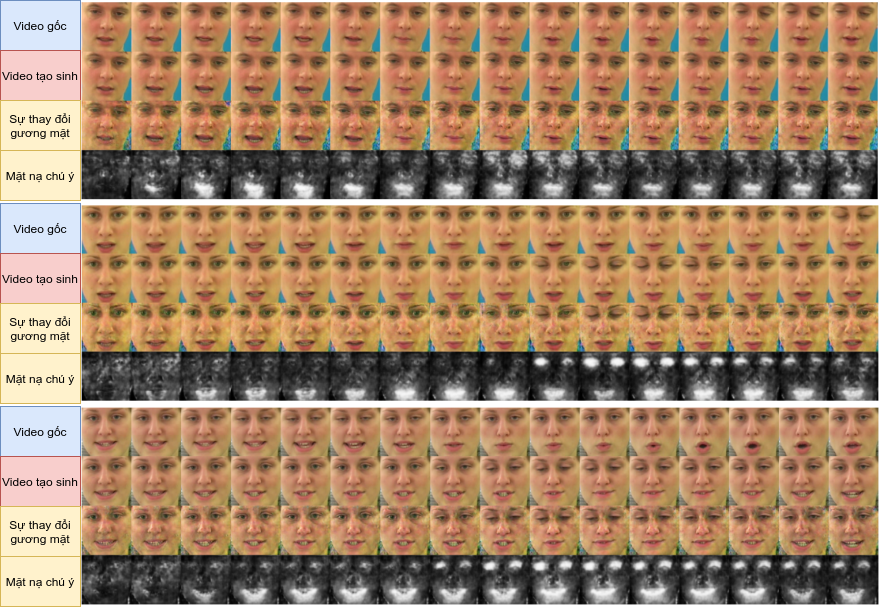
\includegraphics[width=15cm]{./content/materials/grid_examples-face.png}
    \caption{Kết quả tạo sinh gương mặt theo giọng nói trên tập GRID}
\end{figure}

\subsection{Các kết quả trên tập dữ liệu LRW}

Do tập dữ liệu có khối lượng dữ liệu lớn hơn tập GRID nhiều lần và dữ liệu không được chuẩn hóa tốt như tập dữ liệu GRID. Huấn luyện mạng trên tập LRW cũng khó hội tụ hơn và không cho kết quả tốt như tập GRID. Với tập dữ liệu LRW, thời gian huấn luyện là 9 giờ 30 phút cho mỗi vòng lặp qua dữ liệu (tính trên thiết bị đồ họa NVIDIA V100). Mạng hội tụ và cho kết quả tốt nhất sau 25 vòng lặp. Tại thời điểm hội tụ, các hàm mất mát trên mạng có giá trị:

\begin{table}[h]
    \centering
    \begin{tabular}{c | c | c | c | c}
    \hline 
    \multicolumn{5}{c}{LRW}\\
    \hline 
    \textbf{$\mathcal{L}_{landmark}$} & \textbf{$\mathcal{L}_{pix}$} & \textbf{$\mathcal{L}_{gans-dis}$} & \textbf{$\mathcal{L}_{gans-landmark}$} & \textbf{$\mathcal{L}$}\\
    \hline
    $2.012 \times 10^{-4}$ & $6.8502 \times 10^{-2}$ & $0.6931$ & $5.2412 \times 10^{-2}$ & $1.4306$\\
    \hline
    \end{tabular}
    \caption{Các giá trị mất mát của mạng khi hội tụ tại vòng lặp thứ 25}
    \label{table:lrw_loss}
\end{table}

\begin{figure}[H]
    \centering
    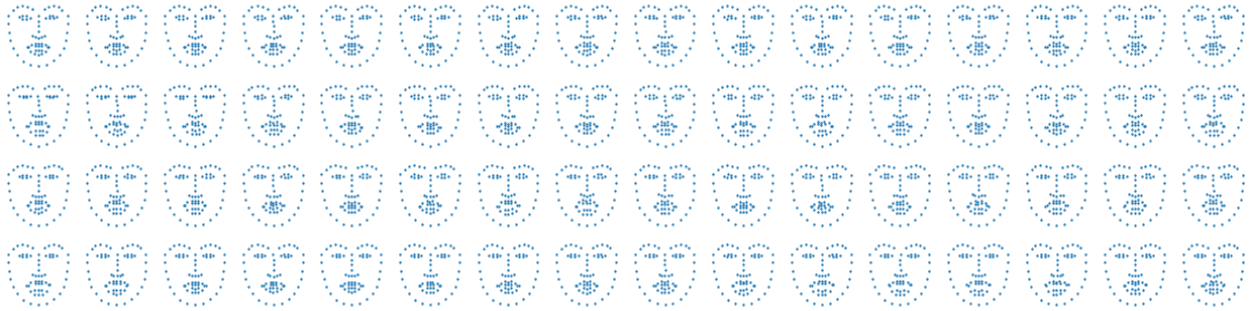
\includegraphics[width=15cm]{./content/materials/lrw_examples-landmark.png}
    \caption{Kết quả tạo sinh cột mốc gương mặt trên tập LRW}
\end{figure}

Hình sau thể hiện kết quả tạo sinh video khi cho mô hình tạo sinh ảnh trên tập kiểm thử với 3 trường hợp: ảnh mẫu được chuẩn hóa tốt, ảnh đầu vào bị lệch, và ảnh đầu vào được quay một bên mặt.

\begin{figure}[H]
    \centering
    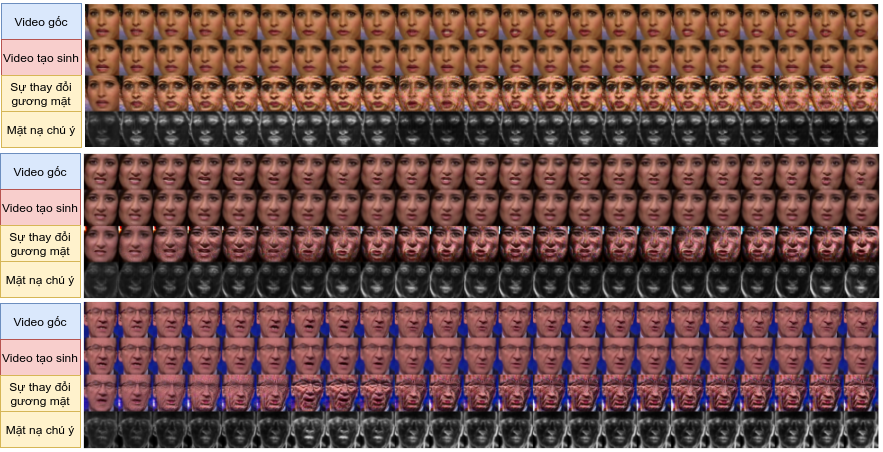
\includegraphics[width=15cm]{./content/materials/lrw_examples-frontal.png}
    \caption{Kết quả tạo sinh gương mặt theo giọng nói trên tập LRW, trường hợp ảnh đầu vào là hình ảnh chiếu thẳng mặt người nói, mặt người được canh bốn góc, mũi nằm ở giữa khung hình}
\end{figure}

\begin{figure}[H]
    \centering
    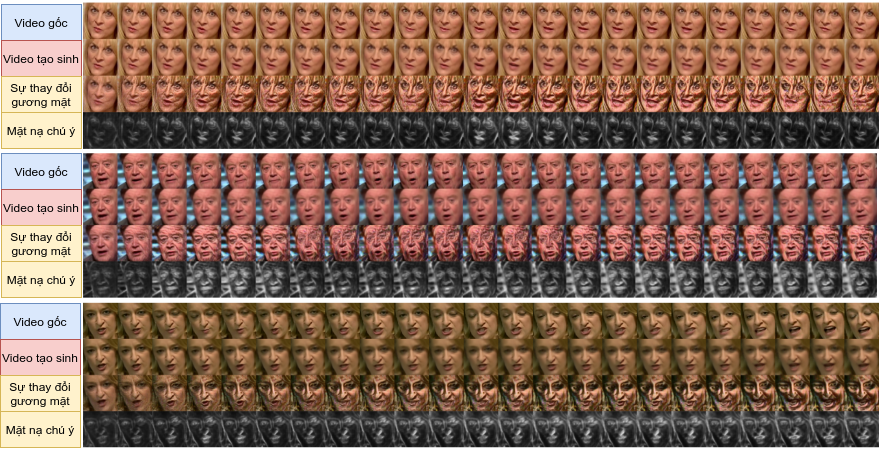
\includegraphics[width=15cm]{./content/materials/lrw_examples-miss_aligned.png}
    \caption{Kết quả tạo sinh gương mặt theo giọng nói trên tập LRW, trường hợp ảnh đầu vào là hình ảnh bị lệch, mặt người nằm ở 1 phía trên khung hình}
\end{figure}

\begin{figure}[H]
    \centering
    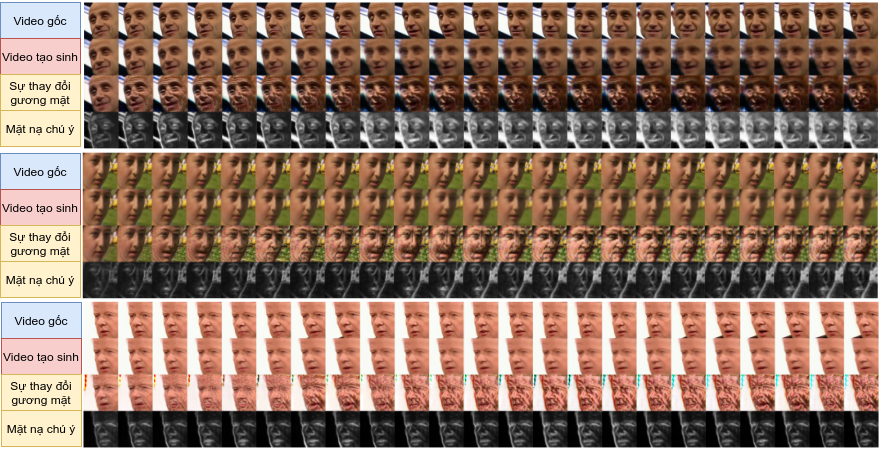
\includegraphics[width=15cm]{./content/materials/lrw_examples-half_face.png}
    \caption{Kết quả tạo sinh gương mặt theo giọng nói trên tập LRW, trường hợp ảnh đầu vào là hình ảnh lệch hẳn về một bên mặt}
\end{figure}

Hình ảnh trên cho thấy, mạng cho kết quả tốt nhất khi tạo sinh ảnh có chứa mặt người mẫu được chụp theo hướng chính diện, mặt người được chuẩn hóa tốt.

\section{\texorpdfstring{Kết luận và hướng nghiên cứu mở rộng đề tài}{conclusion}}
%Mô tả, bình luận ngắn gọn và đưa ra kết luận về kết quả nghiên cứu của luận văn và cách thức áp dụng thực tiễn. Đề ra các hướng nghiên cứu mở rộng cho Luận văn.



% \chapter{Giới thiệu đề tài}
% Nêu lý do chọn đề tài, mục đích, đối tượng và phạm vi nghiên cứu, ý nghĩa khoa học và ý nghĩa thực tiễn của đề tài.

Trong những năm gần đây, với sự bùng nổ và phát triển cực kì mạnh mẽ của ngành công nghệ thông tin và đặc biệt là ngành trí tuệ nhân tạo, ngày càng nhiều các sáng kiến đôc đáo đã được sinh ra. Trong đó, việc tạo sinh dữ liệu tự động sử dụng trí tuệ nhân tạo đã đánh dấu một bước chuyển mình mới và cực kì sáng tạo.

So với các mô hình truyền thống với mục đích phân lớp, phân đoạn, gom nhóm, và dự đoán theo chuỗi thời gian, nhóm các mô hình tạo sinh dữ liệu được sinh ra với mục đích hoàn toàn khác. Trong khi các mô hình truyền thống cung cấp thông tin đã hiện hữu trong thế giới thực (bài toán nhận diện vật thể, OCR, phân đoạn hình ảnh,...) hoặc các dự đoán về các sự kiện sẽ xảy ra (dự đoán giá chứng khoán, dự đoán diễn biến dịch COVID-19,...), thì các mô hình tạo sinh dữ liệu lại cố gắng tạo ra dữ liệu mới, chưa từng tồn tại trong thế giới thực.

Một số ví dụ về việc tạo sinh dữ liệu bằng trí tuệ có thể kể đến như: sử dụng mạng LSTM để sáng tác nhạc, hay công trình chuyển đổi phong cách hình ảnh (style transfer) của giáo sư Fei Fei Li và cộng sự \cite{Johnson2016Perceptual}, hay trang web \url{https://thispersondoesnotexist.com}, được tạo nên để tạo sinh những gương mặt người chưa từng tồn tại bằng mạng StyleGAN2 \cite{stylegans}.

Bài toán tạo sinh dữ liệu dựa trên những nguồn dữ liệu có tính chất khác nhau đã và đang trở thành xu thế trong những năm trở lại đây. Đây là bài toán có tính cấp bách, mang lại giá trị cao về mặt kiến thức cho ngành trí tuệ nhân tạo nói riêng và giá trị về mặt kinh tế, công nghệ chung cho toàn xã hội xã hội. Bên cạnh đó, việc tạo sinh dữ liệu về con người đã đạt được những tiến bộ vượt bậc, đặc biệt là tạo sinh dữ liệu hình ảnh khuôn mặt người.

Kiến trúc mạng Generative Adversarial Network \cite{gans_base} ra đời vào năm 2014 đã đánh dấu một bước chuyển mình mới cho ngành trí tuệ nhân tạo. Kiến trúc này giúp cho việc tạo sinh dữ liệu được thực hiện một cách hiệu quả và chính xác hơn. Dựa trên nền tảng đó, các nghiên cứu về việc tạo sinh ảnh gương mặt người cũng được tiến hành và ngày càng có những bước tiến mới.

\section{\texorpdfstring{Lý do chọn đề tài}{Why}}
Việc tạo sinh hình ảnh khuôn mặt người dựa trên tiếng nói đang là nhu cầu cần thiết trong ngành giải trí, phim ảnh, hoạt hình. Nếu xây dựng được một hệ thống tạo hình khuôn mặt tốt, chi phí sản xuất phim sẽ được giảm thiểu đáng kể vì phần hóa trang có thể được cắt bớt, phần kĩ xảo có thể được đơn giản hóa, diễn viên không phải quá mạo hiểm trong các cảnh quay nguy hiểm. Đối với hoạt hình, phần hình vẽ có thể được hỗ trợ rất nhiều bởi hệ thống tạo sinh khuôn mặt, từ đó có thể giảm bớt chi phí vẽ hình. Bên cạnh đó, ta có thể tạo sinh gương mặt đại diện trong trường hợp người nói không muốn lộ diện. Ngoài những ứng dụng rất hữu ích trong thực tiễn như đã nêu ở trên, bài toán tạo sinh gương mặt còn là một bài toán khó, thú vị và mới mẻ, còn nhiều hướng đi chưa được khai phá và cực kì tiềm năng trong tương lai.

\section{\texorpdfstring{Mục đích của nghiên cứu}{Target}}
Nghiên cứu nhằm mục đích kiểm nghiệm các mô hình được đề xuất trong các nghiên cứu gần đây, tìm hiểu các phương pháp tiền xử lý dữ liệu và trích xuất đặc trưng mới giúp mô hình dễ học hơn, tạo sinh ra hình ảnh chân thật và có độ chính xác cao, khó bị nhận biết bởi con người.

\section{\texorpdfstring{Đối tượng nghiên cứu}{Objective}}
Đối tượng nghiên cứu của Luận văn là các cách tiếp cận, các phương pháp mô hình hóa bài toán, các mạng học máy, học sâu, mạng GANs và các phương pháp tạo sinh dữ liệu từ mạng GANs, các cấu trúc Residual Encoder-Decoder, bên cạnh đó là các phương pháp kết hợp đặc trưng hình ảnh, âm thanh có xem xét đến thứ tự thời gian để tạo sinh hình ảnh mới.

\section{\texorpdfstring{Phạm vi nghiên cứu}{Research}}
Phạm vi nghiên cứu của Luận văn là tạo sinh ảnh giới hạn trong vùng mặt của người, dữ liệu mẫu được cung cấp ban đầu phải là ảnh rõ ràng của khuôn mặt người, đoạn âm thanh được cung cấp cũng phải là âm thanh rõ ràng của tiếng nói.

\section{\texorpdfstring{Ý nghĩa khoa học}{ScientificMeaning}}
Đóng góp cho sự phát triển chung của xu hướng tạo sinh dữ liệu mới dựa trên các tính chất của dữ liệu ban đầu. Việc tìm ra phương pháp giải quyết tốt bài toán sẽ tạo nên tảng để giải quyết những bài toán xa hơn, phức tạp hơn như: tạo sinh nửa người trên, tạo sinh toàn bộ cơ thể người, hay tạo sinh cả một bối cảnh trong phim. Đề tài giúp kiểm chứng, hiện thực, thử nghiệm các phương pháp hiện có trong các bài nghiên cứu gần đây, so sánh và tổng hợp để cố gắng tìm ra hướng đi mới, đóng góp thêm phương pháp mới cho việc tạo sinh ảnh. Đồng thời, các phương pháp tạo sinh dữ liệu cũng giúp làm giàu dữ liệu để huấn luyện, kiểm thử cho các mô hình học máy, học sâu khác.

\section{\texorpdfstring{Ý nghĩa thực tiễn}{RealLifeMeaning}}
Giải quyết thành công vấn đề này đem lại giá trị to lớn về mặt công nghệ, kinh tế và xã hội. Chúng ta có thể tái hiện lại gương mặt người đang nói ở nhiều thứ tiếng khác nhau, tạo sinh khuôn mặt người đại diện trong các hội nghị trực tuyến, tích hợp vào các trò chơi điện tử để làm chúng trở nên chân thực hơn, truyền video trong điều kiện băng thông giới hạn, giả lập trợ lý ảo có hình dáng con người,... Đối với ngành truyền thông, nó có thể tạo ra biên tập viên ảo. Đối với ngành điện ảnh, giải trí, sáng tạo nội dung nó cũng có giá trị ứng dụng khi giúp giảm bớt áp lực lên khâu hóa trang, kỹ xảo.

% \include{./content/III}
% \include{./content/IV}
% \chapter{Kết quả nghiên cứu}
%Mô tả ngắn gọn các kết quả nghiên cứu, thực nghiệm. Bàn luận về điểm mạnh, điểm yếu của mô hình được xây dựng trong luận văn. So sánh kết quả thu được trong quá trình nghiên cứu, thực nghiệm của đề tài và đối chiếu với kết quả nghiên cứu, thực nghiệm của các tác giả khác một cách khách quan. Nêu lên điểm nổi bật, khác biệt của luận văn đối với các nghiên cứu khác.

\section{Các tập dữ liệu được sử dụng}
\subsection{Tập dữ liệu LRW \cite{lrw}}

Tập dữ liệu LRW là tập dữ liệu được xây dựng bởi một nhóm nghiên cứu từ trường Đại học Oxford và sở hữu bởi hãng tin tức BBC. Đây là tập dữ liệu lớn, với những đoạn video ngắn được cắt từ những đoạn video được phát trên kênh BBC và được thu trong môi trường tự nhiên. Tập dữ liệu LRW có hơn 1 triệu video khác nhau, mỗi video có độ dài 1.16 giây, gồm 29 khung hình. Những video này được chia làm 1000 từ vựng, mỗi từ vựng được nói bởi hơn 1000 người khác nhau. Tổng cộng, tập dữ liệu LRW chứa gần 1000 giờ video. Tuy nhiên, do được thu trong môi trường tự nhiên, tín hiệu trong video có độ nhiễu nhất định. Âm thanh trong video có thể nghe rõ lời nói, tuy nhiên một số lượng không nhỏ video bị lẫn tiếng ồn và các tạp âm khác. Về mặt hình ảnh, video có hình ảnh rõ nét, lấy điểm trên đầu mũi của người đang nói làm trung tâm, vì vậy, với các video mà người nói có sự cử động ở đầu như xoay hay lắc đầu, video sẽ bị rung lắc mạnh để giữ điểm đầu mũi ở giữa khung hình. Mặt người trong video được quay ở nhiều vị trí khác nhau và có thể lệch về một phía (quay từ phía bên trái, bên phải, hoặc lệch theo chiều dọc gương mặt). Với mỗi từ ngữ, tập dữ liệu đã chia sẵn thành 3 tập tập huấn luyện, tập kiểm chứng và tập kiểm thử với số lượng video tương ứng cho mỗi loại là 1000-50-50.

\begin{figure}[H]
    \centering
    \includegraphics[width=12cm]{./content/materials/lrw.png}
    \caption{Ảnh trích xuất từ các video trong tập dữ liệu LRW}
\end{figure}

\subsection{Tập dữ liệu GRID \cite{grid}}

Tập dữ liệu GRID là tập dữ liệu được tạo ra từ phòng nghiên cứu của Đại học Sheffield tại Anh. Tập dữ liệu này được tạo ra để hỗ trợ cho việc phân tích và nghiên cứu gương mặt người khi nói, bao gồm các nghiên cứu về nhận thức gương mặt thông qua giọng nói và nhận diện giọng nói. Tập dữ liệu chứa 1000 câu, được nói bởi 34 người khác nhau. Như vậy, tập dữ liệu này chứa 34000 video với chất lượng cao, mỗi video có độ dài 3 giây. Những câu được nói rất đơn giản, với cú pháp: <động từ (4 từ)> <màu sắc (4 từ)> <giới từ (4 từ)> <chữ cái (25 chữ)> <số (10 số)> <trạng từ (4 từ)>. Các cụm từ giống hệt nhau về mặt cú pháp đã nêu ở trên (ví dụ như câu "place green at B 4 now"), được phát âm rõ và đọc với tốc độ bình thường, âm thanh được thu ở môi trường kín, không nhiễu. Hình ảnh trong video rõ nét, được quay với phông nền xanh với điều kiện ánh sáng tốt. Mặt người khi nói ít chuyển động (ít xoay, ít lắc đầu) và được quay trực diện. Gương mặt người khi nói không biểu lộ cảm xúc và người nói chớp mắt một cách tự nhiên. Các video trong tập GRID được chia thành 3 tập huấn luyện, tập kiểm chứng và tập kiểm thử với tỉ lệ 90\%-5\%-5\% tương ứng.

Do tập dữ liệu LRW có độ nhiễu cao, nên ta sẽ sử dụng tập dữ liệu GRID để tính cột mốc gương mặt chuẩn $l_{standard}$ như đã miêu tả ở phân \ref{sec:preprocess_audio_lm}. Cột mốc gương mặt chuẩn $l_{standard}$ tuy được tính toán trên tập GRID nhưng sẽ được sử dụng để chuẩn hóa cột mốc gương mặt cho cả tập GRID và tập LRW. Cách thức chuẩn hóa cột mốc khuôn mặt trong luận văn lấy ý tưởng từ bài báo \cite{gen_face_landmark} và được chỉnh sửa để phù hợp với việc xử lý dữ liệu cho bài toán.

\begin{figure}[H]
    \centering
    \includegraphics[width=12cm]{./content/materials/grid.png}
    \caption{Ảnh trích xuất từ các video trong tập dữ liệu GRID}
\end{figure}

\section{Các độ đo được sử dụng để đánh giá kết quả tạo sinh hình ảnh}\label{sec:metrics}

Việc tạo sinh dữ liệu hình ảnh mặt người dựa theo giọng nói hiện tại vẫn chưa có một độ đo nào làm chuẩn mực để đánh giá chất lượng tạo sinh hình ảnh, thậm chí một số nghiên cứu về vấn đề này trên các tạp chí uy tín cũng được xuất bản mà không có độ đo chuẩn để đánh giá mô hình một cách cụ thể \cite{chung} \cite{wav2pix}.

Một video mặt người đang nói trong tự nhiên có thể có các chuyển động đầu, mắt, và biểu cảm gương mặt tùy ý. Tuy nhiên video được tạo sinh có thể có thể tạo ra chuyển động đầu theo một hướng khác, chớp mắt ở thời điểm khác và biểu cảm gương mặt theo một cách khác. Vì vậy một độ đo lý tưởng là một độ đo không bị ảnh hưởng bởi các chuyển động của đầu, chớp mắt và biểu cảm gương mặt mà nên tập trung vào nội dung và bản chất của hình ảnh. Việc sử dụng hàm mất mát L2 trong việc tạo sinh ảnh có thể làm cho hình ảnh ổn định và đẹp hơn, tuy nhiên khó có thể dùng hàm mất mát L2 để đánh giá hình ảnh tạo sinh một cách công bằng do hàm mất mát L2 sẽ gây ra giá trị mất mát lớn nếu chuyển động của đầu trong video được tạo sinh không giống với video gốc. Ta có thể dùng độ đo PSNR (Peak Signal-to-Noise) để tính toán độ sai lệch cho từng điểm ảnh dựa vào hàm mất mát L2. Tuy nhiên, như đã giải thích ở trên, độ đo này bỏ qua tính tự nhiên trong quá trình chuyển động của đầu và gương mặt trong ảnh tạo sinh mà chỉ chú trọng vào sự giống nhau ở từng điểm ảnh trên video gốc vào video tạo sinh. Vì vậy đây không phải là một độ đo thật sự tốt để đánh giá chất lượng tạo sinh hình ảnh.

Một độ đo tốt hơn PSNR cho việc tính toán sự tương đồng giữa video gốc và video tạo sinh là SSIM (structural similarity index measure) \cite{ssim}. Độ đo này được sử dụng để đo sự tương đồng về mặt cấu trúc giữa hai hình ảnh, nhằm giảm bớt sự cứng nhắc của các phép so sánh chính xác \cite{psrn_ssim}. Độ đo này được tính toán bằng cách so sánh các điểm ảnh xung quanh của một điểm ảnh trên ảnh gốc và ảnh được tạo sinh với ba kênh gồm kênh tương phản, kênh độ chói và kênh cấu trúc. Ý tưởng về mặt so sánh cấu trúc giữa hai hình ảnh được đưa ra từ việc một điểm ảnh sẽ luôn có sự liên kết chặt chẽ với các điểm ảnh xung quanh nó. Sự liên kết này hàm chứa thông tin quan trọng về cấu trúc của những vật thể trong ảnh. Bên cạnh đó, độ đo này cũng lưu ý đến sự chói sáng và sự khác biệt về độ tương phản của ảnh trong những vùng có sự thay đổi. Hình sau là một ví dụ so sánh giữa sai số L2 và SSIM:

\begin{figure}[H]
    \centering
    \includegraphics[width=15cm]{./content/materials/l2_ssim.png}
    \caption{So sánh giữa sai số L2 và SSIM}
\end{figure}

Để đo lường độ sắc nét của hình ảnh được tạo sinh, ta sử dụng độ đo CPBD (Cumulative 
Probability of Blur Detection) \cite{cpbd}. Bằng cách kết hợp ý tưởng của việc phát hiện vùng mờ bằng xác suất tích lũy với định nghĩa về vùng mờ vừa được chú ý (just noticeable blur) thành một mô hình tổng hợp xác suất, CPBD đánh giá độ sắc nét của hình ảnh trên quan điểm tri giác, phù hợp với nhận thức của con người.

Trong luận văn này, ta sử dụng SSIM để đo lường chất lượng hình ảnh của video được tạo sinh và CPBD để đo lường độ sắc nét cho các khung hình

\section{Quá trình thực hiện}

Chi tiết các môi trường huấn luyện và chạy các thí nghiệm được liệt kê ở bảng \ref{table:hardware}

\begin{table}[h]
    \centering
    \begin{tabular}{c | c | c}
    \hline 
    &\textbf{Máy A} & \textbf{Máy B}\\
    \hline
    \textbf{CPU} & Intel Xeon & Intel Core I5 8600K\\
    \textbf{Bộ nhớ} & 24GB & 32GB\\
    \textbf{GPU} & NVIDIA TESLA V100 & NVIDIA Geforce RTX 3070\\
    \textbf{Ổ cứng} & 160GB SSD & 768GB NVME SSD + 2TB HDD\\
    \textbf{OS} & N/A(Colab Pro) & Ubuntu 20.04\\
    \textbf{Ngôn ngữ} & Python 3.7 & Python 3.7\\
    \textbf{Framework} & Pytorch 1.8 & Pytorch 1.8\\
    \hline
    \end{tabular}
    \caption{Các môi trường được sử dụng trong việc tiền xử lý dữ liệu, huấn luyện và thực hiện thí nghiệm}
    \label{table:hardware}
\end{table}

Máy A được sử dụng trong việc huấn luyện hệ thống mạng GANs bao gồm mạng tạo sinh hình ảnh và mạng phân biệt. Trong khi máy B được sử dụng để làm những công đoạn còn lại bao gồm tiền xử lý dữ liệu, huấn luyện mạng tạo sinh cột mốc gương mặt và tiến hành chạy các thí nghiệm, đo đạc thông số. Các số liệu sau đây đều được ghi nhận trên các thiết bị này. 

Việc huấn luyện mạng như đã nói được chia làm hai bước. Bước đầu tiên là huấn luyện mạng tạo sinh cột mốc gương mặt và bước thứ hai là huấn luyện hệ thống mạng GANs. Các thông số và kết quả huấn luyện mạng tạo sinh cột mốc gương mặt trên máy B cho hai tập dữ liệu được thể hiện qua bảng sau:

\begin{table}[h]
    \centering
    \begin{tabular}{c | c | c}
    \hline 
    &\textbf{GRID} & \textbf{LRW}\\
    \hline
    \textbf{Bộ tối ưu} & Adam & Adam\\
    \textbf{Kích thước bó} & 100 & 100\\
    \textbf{Hệ số học} & 0.001 & 0.0002\\
    \textbf{Thời gian huấn luyện} & 5 phút & 70 phút\\
    \textbf{$\mathcal{L}_{landmark}$} & $4.9200 \times 10^{-4}$ & $2.012 \times 10^{-4}$\\
    \hline
    \end{tabular}
    \caption{Chi tiết huấn luyện mạng tạo sinh cột mốc gương mặt. Giá trị mất mát (trên tập kiểm thử) và thời gian huấn luyện được ghi nhận tại vòng lặp cho ra mô hình tối ưu}
    \label{table:landmark_decoder_training_detail}
\end{table}

Mạng tạo sinh cột mốc gương mặt có cấu trúc đơn giản và huấn luyện nhanh. Do tập dữ liệu LRW có kích thước rất lớn và cấu trúc dữ liệu phức tạp hơn nên ta cái đặt hệ số học nhỏ hơn. Đồng thời thời gian huấn luyện mạng này cùng lâu hơn mạng GRID nhiều lần. Tuy nhiên mạng này cho ra giá trị mất mát MSE nhỏ hơn do có nhiều dữ liệu để học hơn. Bước thứ hai trong việc huấn luyện mạng là huấn luyện hệ thống mạng GANs. Việc huấn luyện này được tiến hành trên máy A. Chi tiết về việc huấn luyện mạng được liệt kê trong bảng sau:

\begin{table}[h]
    \centering
    \begin{tabular}{c | c | c}
    \hline 
    &\textbf{GRID} & \textbf{LRW}\\
    \hline
    \textbf{Bộ tối ưu} & Adam & Adam\\
    \textbf{Kích thước bó} & 12 & 17\\
    \textbf{Hệ số học} & 0.0002 & 0.0002\\
    \textbf{Thời gian huấn luyện} & 5 giờ 20 phút & 250 giờ\\
    \textbf{$\mathcal{L}_{pix}$} & $4.1575 \times 10^{-2}$ & $6.8502 \times 10^{-2}$\\
    \textbf{$\mathcal{L}_{gans-dis}$} & $0.9964$ & $0.6931$\\
    \textbf{$\mathcal{L}_{gans-landmark}$} & $7.6990 \times 10^{-2}$ & $5.2412 \times 10^{-2}$\\
    \textbf{$\mathcal{L}$} & $1.4892$ & $1.4306$\\
    \hline
    \end{tabular}
    \caption{Chi tiết huấn luyện mạng GANs. Giá trị mất mát (trên tập kiểm thử) và thời gian huấn luyện được ghi nhận tại vòng lặp cho ra mô hình tối ưu}
    \label{table:gans_training_detail}
\end{table}

Theo như bảng trên, việc huấn luyện mạng GANs cho tập dữ liệu LRW có thời gian rất lâu, mạng này được huấn luyện đến vòng lặp thứ 25 (mỗi vòng lặp khoảng 10 giờ) thì hội tụ. Tuy nhiên tác giả đã huấn luyện thêm đến vòng lặp thứ 40 để chắc chắn không rơi vào vùng tối ưu cục bộ. Các giá trị hàm mất mát cho thấy giá trị mất mát tổng ở cả hai tập GRID và LRW ($\mathcal{L}$) là gần bằng nhau. Tuy nhiên, trong các giá trị mất mát thành phần thì giá trị $\mathcal{L}_{gans-landmark}$ và $\mathcal{L}_{gans-dis}$ ở tập LRW có giá trị thấp hơn do tập LRW có nhiều dữ liệu hơn để học, nên mạng phân biệt của tập LRW có khả năng phân biệt thật giả và sinh ra cột mốc gương mặt tốt hơn hẳn so với tập GRID. Ngược lại, ở tập GRID, giá trị $\mathcal{L}_{pix}$ của tập này thấp hơn so với tập LRW do tính chất dữ liệu của nó. Đối với tập GRID, như đã nói, các video trong tập này được quay trong phòng thí nghiệm và được canh chỉnh sao cho gương mặt không xoay và không di chuyển. Vì vậy mạng dễ học để tạo sinh chính xác hình ảnh hơn để có hàm mất mát L1 thấp hơn hẳn tập LRW.


\section{Các kết quả trên tập dữ liệu GRID}

Đầu tiên, ta thử tạo sinh cột mốc gương mặt từ giọng nói sử dụng mạng tạo sinh cột mốc gương mặt vừa được huấn luyện ở các bước trên. Kết quả tạo sinh cột mốc gương mặt được thể hiện ở hình dưới.

\begin{figure}[H]
    \centering
    \includegraphics[width=15cm]{./content/materials/grid_examples-landmark.png}
    \caption{Kết quả tạo sinh cột mốc gương mặt trên tập GRID, cột mốc màu đỏ là cột mốc được tạo sinh, màu xanh là cột mốc được trích xuất từ hình ảnh gốc}
\end{figure}

So sánh cột mốc gương mặt được tạo sinh (cột mốc màu đỏ) và cột mốc gốc (màu xanh) ta thấy mạng đã dự đoán tương đối tốt chuyển động của cột mốc gương mặt theo lời nói dựa vào độ trùng lắp của các cột mốc. Ta đưa các cột mốc vừa được tính toán vào mạng tạo sinh kèm với hình ảnh mẫu và cột mốc gương mặt của ảnh mẫu, ta sẽ tạo ra được chuỗi hình ảnh mặt người đang nói. Mạng phân biệt sẽ không được sử dụng trong quá trình sinh ảnh này. Sau đây là một số ví dụ tạo sinh ảnh trên tập GRID

\begin{figure}[H]
    \centering
    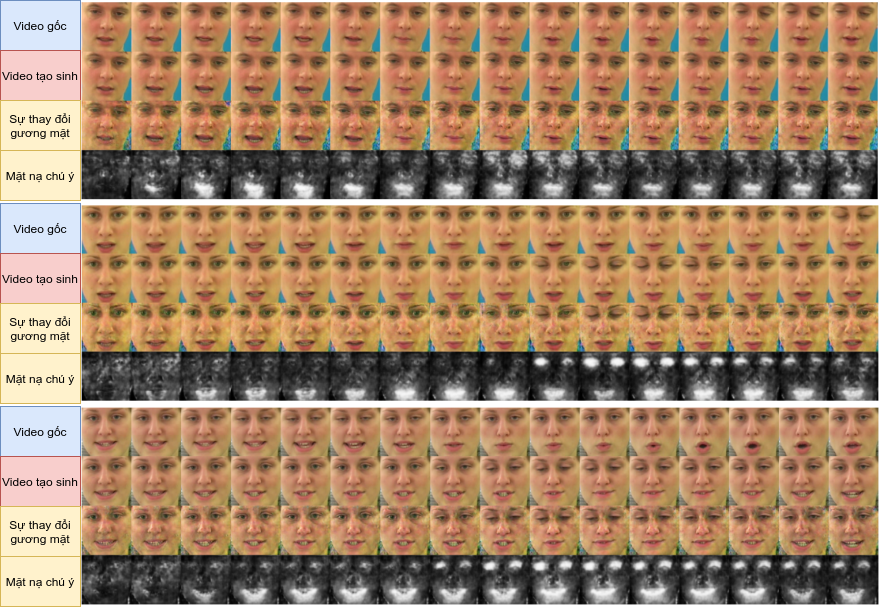
\includegraphics[width=15cm]{./content/materials/grid_examples-face.png}
    \caption{Kết quả tạo sinh gương mặt theo giọng nói trên tập GRID}
\end{figure}

Theo kết quả tạo sinh ta thấy, hình ảnh tạo sinh có khẩu hình miệng phù hợp với tiếng nói và gần giống với video gốc. Mặt nạ chú ý chủ yếu tập trung vào vùng mắt và miệng, trong khi các phần khác trên gương mặt và phông nền dường như không được chú ý đến. Một số video ngoài khả năng cử động miệng, có thể sinh ra hành động chớp mắt và hành động này diễn ra một cách ngẫu nhiên. Hành động chớp mắt diễn ra trong vòng 6 đến 7 khung hình, tương ứng với khoảng thời gian 240ms đến 280ms, phù hợp với hành động chớp mắt trong thực tế của con người. Trên video mô tả sự thay đổi gương mặt $p'_{image}$, chỉ có các vùng được chú ý đến mới được tạo sinh hình ảnh rõ ràng, các vùng còn lại thường sinh ra nhiễu. Điều này rất hợp lý vì trên thực tế, các vùng không được chú ý đến sẽ không đóng góp nhiều vào giá trị mất mát của mạng, nên những vùng này cũng không cần được tạo sinh một cách hoàn chỉnh.

Tác giả cũng đã chạy thử để tạo sinh hình ảnh gương mặt người đang nói trong điều kiện ảnh thực tế. Hình ảnh sau là ảnh người mẫu được thử nghiệm và kết quả tạo sinh thực tế cho đoạn âm thanh với câu nói: "set red by z5 soon".
\begin{figure}[H]
    \centering
    \includegraphics[width=5cm]{./content/materials/khang.png}
    \caption{Ảnh người mẫu trong thử nghiệm chạy thực tế}
\end{figure}

\begin{figure}[H]
    \centering
    \includegraphics[width=16cm]{./content/materials/khang_gen.png}
    \caption{Video được tạo sinh bởi mô hình GRID}
\end{figure}

Ta thấy mặc dù bị gây nhiễu bởi khẩu trang và kính, nhưng mô hình vẫn tạo sinh được video có chất lượng tương đối tốt và vẫn giữ nguyên được đặc trưng gương mặt người nói. Phần được chú ý chủ yếu vẫn là phần miệng, chuyển động của miệng tương đồng với từ ngữ được nói trong đoạn âm thanh.

\section{Các kết quả trên tập dữ liệu LRW}
Tiến hành các bước tạo sinh tương tự như trên tập dữ liệu GRID, ta thu được các kết quả tạo sinh cột mốc gương mặt tốt hơn so với tập GRID. Điều này đã được giải thích ở phần trên, do tập LRW là tập dữ liệu rất lớn, nên mạng có nhiều dữ liệu hơn để học về âm thanh và cột mốc gương mặt.

\begin{figure}[H]
    \centering
    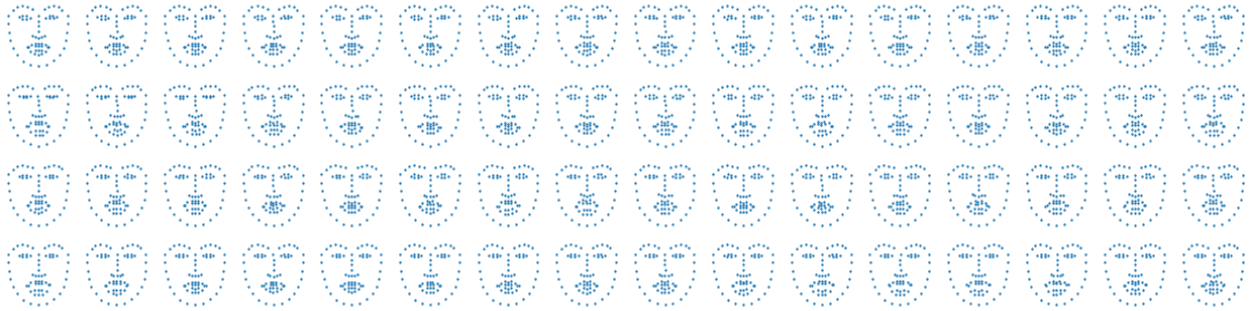
\includegraphics[width=15cm]{./content/materials/lrw_examples-landmark.png}
    \caption{Kết quả tạo sinh cột mốc gương mặt trên tập LRW, cột mốc màu đỏ là cột mốc được tạo sinh, màu xanh là cột mốc được trích xuất từ hình ảnh gốc}
\end{figure}

Hình sau thể hiện kết quả tạo sinh video khi cho mô hình tạo sinh ảnh trên tập kiểm thử với 3 trường hợp: ảnh mẫu được chuẩn hóa tốt, ảnh đầu vào bị lệch, và ảnh đầu vào được quay một bên mặt.

\begin{figure}[H]
    \centering
    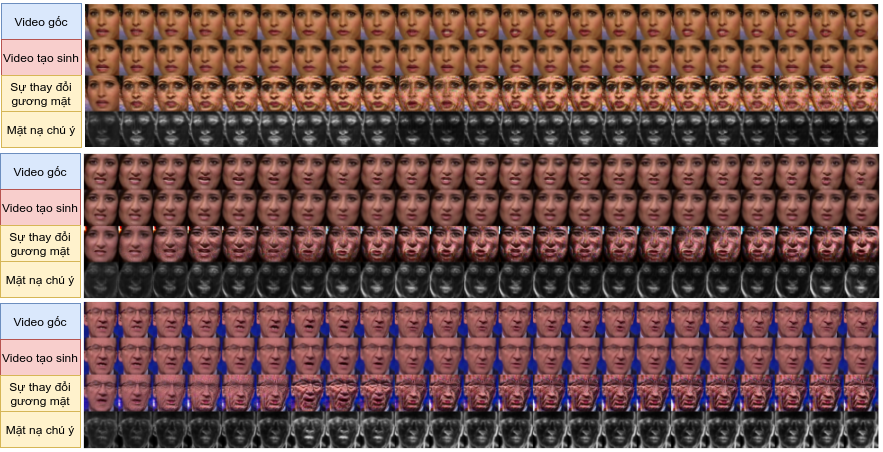
\includegraphics[width=15cm]{./content/materials/lrw_examples-frontal.png}
    \caption{Kết quả tạo sinh gương mặt theo giọng nói trên tập LRW, trường hợp ảnh đầu vào là hình ảnh chiếu thẳng mặt người nói, mặt người được canh bốn góc, mũi nằm ở giữa khung hình}
\end{figure}

\begin{figure}[H]
    \centering
    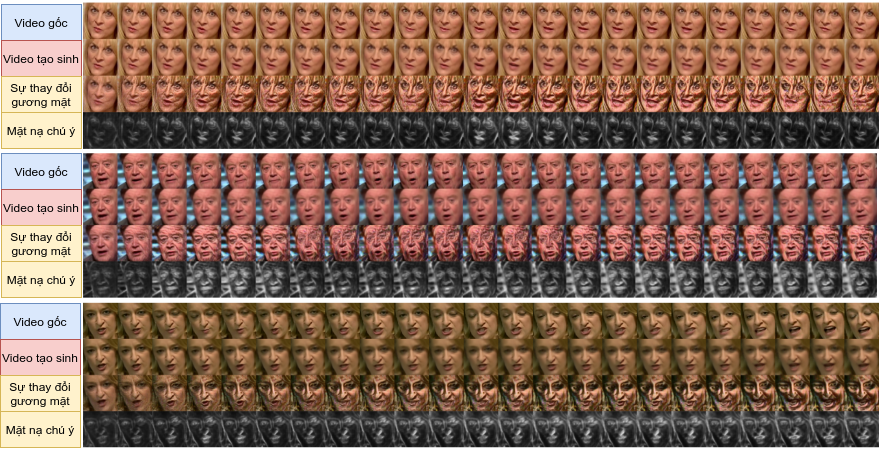
\includegraphics[width=15cm]{./content/materials/lrw_examples-miss_aligned.png}
    \caption{Kết quả tạo sinh gương mặt theo giọng nói trên tập LRW, trường hợp ảnh đầu vào là hình ảnh bị lệch, mặt người nằm ở 1 phía trên khung hình}
\end{figure}

\begin{figure}[H]
    \centering
    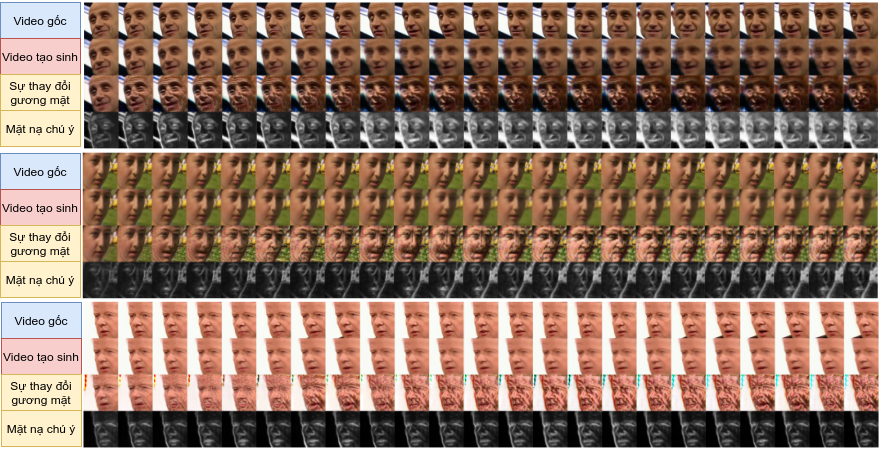
\includegraphics[width=15cm]{./content/materials/lrw_examples-half_face.png}
    \caption{Kết quả tạo sinh gương mặt theo giọng nói trên tập LRW, trường hợp ảnh đầu vào là hình ảnh lệch hẳn về một bên mặt}
\end{figure}

Hình ảnh trên cho thấy, giống như trong tập dữ liệu GRID, phần mắt và miệng trên gương mặt là phần được chú ý nhiều nhất. Các phần khác của khuôn mặt trong hình  $p'_{image}$ cũng không được tạo sinh một cách hoàn chỉnh. Tuy nhiên, do tập dữ liệu LRW có góc quay rất đa dạng nên khi tạo sinh hình ảnh ở nhiều góc độ khác nhau của gương mặt, ta thấy mạng cho kết quả tốt nhất khi tạo sinh ảnh mặt người mẫu được chụp theo hướng chính diện, mặt người được chuẩn hóa tốt và lấp đầy khung hình. Cũng do sự đa dạng của góc quay trên tập LRW, mạng đã không học được cách chớp mắt như trong mô hình của tập GRID.

Tác giả cũng đã thử tạo sinh video với hình ảnh thực tế trên mô hình này và mang lại kết quả khả quan. Hình ảnh người mẫu và video tạo sinh cho câu nói "set white to g2 please" được thể hiện ở hai hình sau:

\begin{figure}[H]
    \centering
    \includegraphics[width=5cm]{./content/materials/eny.png}
    \caption{Ảnh người mẫu trong thử nghiệm chạy thực tế}
\end{figure}

\begin{figure}[H]
    \centering
    \includegraphics[width=16cm]{./content/materials/eny_gen.png}
    \caption{Video được tạo sinh bởi mô hình LRW}
\end{figure}

Qua thử nghiệm trên ta thấy, mô hình đã tạo sinh tương đối tốt hình ảnh người mẫu đang phát âm các từ ngữ trong câu. Khẩu hình miệng được tạo sinh khớp với âm thanh, mặt người mẫu không bị biến dạng và vẫn giữ được đặc trưng khuôn mặt theo thời gian. Khi thử nghiệm hình ảnh của gương mặt này trên mô hình của tập GRID, video được tạo sinh  có chất lượng không tốt, hình ảnh tạo sinh có chuyển động nhưng những chuyển động này không hợp lý. Điều này có thể giải thích là do khối lượng dữ liệu trên mô hình GRID quá ít, nên mạng chưa có đủ thông tin để tổng quát hóa bài toán cho mọi đầu vào.

\section{So sánh mô hình với các nghiên cứu khác}\label{sec:comparision}

Như đã trình bày ở phần \ref{sec:metrics}, ta sẽ sử dụng độ đo SSIM và CPBD để đánh giá và so sánh mô hình trong nghiên cứu này với các mô hình khác trên hai tập dữ liệu GRID và LRW. Bảng \ref{table:metrics_result} cho thấy phép đo đạc và so sánh giữa các mô hình tạo sinh hình ảnh bằng âm thanh.

\begin{table}[h]
    \centering
    \begin{tabular}{c | c | c | c | c}
    \hline 
    \multirow{2}{*}{\textbf{Phương pháp}} & \multicolumn{2}{c|}{\textbf{GRID}} & \multicolumn{2}{c}{\textbf{LRW}}\\
    \cline{2-5}
    & SSIM & CPBD & SSIM & CPBD\\
    \hline
    \textbf{Zakharov et al \cite{zakharov}} & 0.54 & 0.19 & 0.42 & 0.11 \\
    \textbf{Chung et al \cite{chung}} & 0.41 & \textbf{0.22} & 0.34 & \textbf{0.21} \\
    \textbf{Baseline (Chen et al) \cite{chen2019}} & 0.41 & 0.08 & 0.38 & 0.07 \\
    \hline
    \hline
    \textbf{Ours} & \textbf{0.72} & 0.12 & \textbf{0.54} & 0.06 \\
    \hline
    \end{tabular}
    \caption{So sánh với các mạng có cùng mục tiêu về độ đo SSIM và CPBD. Dữ liệu trong bảng được lấy từ bài khảo sát \cite{chen_survey}}
    \label{table:metrics_result}
\end{table}

Qua bảng \ref{table:metrics_result} ta thấy, việc áp dụng và chỉnh sửa phương pháp chuẩn hóa cột mốc gương mặt từ nghiên cứu \cite{gen_face_landmark} vào mô hình của nghiên cứu \cite{chen2019} đã mang lại hiệu quả tốt. Việc chuẩn hóa đầu vào khi tạo sinh cột mốc gương mặt giúp làm tăng độ đo SSIM lên đáng kể, điều này có nghĩa là so với phương pháp cũ, video được tạo sinh giờ đây có cấu trúc tương đồng hơn với video gốc về mặt cảm quan. Chuyển động của mắt, miệng và cả gương mặt trong video tạo sinh có độ ăn khớp với video gốc cao hơn đáng kể so với các nghiên cứu khác. Nhận diện gương mặt người nói trong video tạo sinh cũng được giữ nguyên và không bị biến dạng, các đặc điểm và chi tiết trên gương mặt vẫn được giữ nguyên so với hình ảnh người mẫu ban đầu.

Do việc tạo sinh một cột mốc gương mặt chuẩn và chính xác là tiền đề rất quan trọng trong việc tạo sinh hình ảnh. Cột mốc gương mặt cũng quyết định phần nhiều khẩu hình miệng khi nói, nên việc chuẩn hóa tốt hơn cột mốc gương mặt ở mạng sinh cột mốc là yếu tố then chốt, ảnh hưởng trực tiếp đến kết quả tạo sinh hình ảnh. Nghiên cứu \cite{chen2019} có sử dụng phương pháp chuẩn hóa, nhưng phương pháp này vẫn còn đơn giản và chủ yếu dựa vào phép biến đổi PCA để loại bỏ các chuyển động không mong muốn trên gương mặt (như lắc, xoay đầu làm cho mắt, mũi miệng bị dịch chuyển mạnh). Trong khi đó, với phương pháp được đề xuất trong luận văn, những chuyển động không mong muốn trên được loại bỏ ngay tại bước tiền xử lý qua các phép biến đổi được nêu ở phần \ref{sec:preprocess_audio_lm}. Điều này giúp cho hệ thống mạng GANs ở phía sau có được thông tin chuẩn xác hơn, dễ học hơn để làm cơ sở cho việc tạo sinh gương mặt người nói.

Tuy nhiên, việc chuẩn hóa video đầu vào có thể được thực hiện chưa được tốt trên tập LRW. Trên thực tế, một số video sau khi được chuẩn hóa trên tập LRW có hiện tượng bị nhảy hình, làm đứt gãy tính thời gian của video và làm cho nó trở nên không được mượt mà. Điều này kết hợp với việc sử dụng hàm mất mát L1 cho bộ tạo sinh hình ảnh làm cho video được tạo sinh trên mô hình của tập LRW không có độ nét tốt (CPBD = 0.06), nhất là những video có góc quay gương mặt lệch hẳn về một bên. Đối với tập dữ liệu GRID có tính ổn định về mặt chuyển động của khung hình, CPBD tăng đáng kể.

% \chapter{Kết luận}
%Mô tả, bình luận ngắn gọn và đưa ra kết luận về kết quả nghiên cứu của luận văn và cách thức áp dụng thực tiễn. Đề ra các hướng nghiên cứu mở rộng cho Luận văn.

Với các cải tiến trong việc chuẩn hóa dữ liệu được đưa ra cho phương pháp tạo sinh ảnh từ bài báo \cite{chen2019}, nghiên cứu này đã đưa ra giải pháp để làm cho hình ảnh được tạo sinh trở nên chính xác hơn và phần nào cải thiện được độ sắc nét của hình ảnh trong tập dữ liệu GRID. Kết quả của nghiên cứu này là một sự cải thiện đáng kể so với mô hình gốc của tác giả Lele Chen. Tuy nhiên, độ sắc nét của hình ảnh vẫn còn thua kém khá xa so với các nghiên cứu cùng thời. So sánh với các nghiên cứu mới nhất ở thời điểm hiện tại, phương pháp được đề xuất vẫn còn khá đơn giản và có kết quả tạo sinh kém hơn hẳn và không miêu tả được chuyển động của đầu, cũng như không tái hiện được khung cảnh xung quanh. Tuy vậy, các nghiên cứu được nói đến ở trên dùng rất nhiều tài nguyên tính toán và khó có thể thực hiện trong điều kiện hiện tại của tác giả.

Trong những năm gần đây, việc tạo sinh hình ảnh gương mặt bắt đầu có nhiều ứng dụng hơn trong thực tiễn cuộc sống. Việc tạo ra phóng viên, biên tập viên truyền hình ảo đang trở nên cần thiết hơn bao giờ hết khi nó có thể tiết kiệm cực kì nhiều chi phí cho đài truyền hình. Chương trình thời sự có thể được truyền đi mà không cần hình ảnh nếu thiết bị đầu cuối có khả năng tạo sinh hình ảnh. Nhờ đó, thời gian truyền thông tin đi cũng nhanh hơn và ít tốn băng thông đường truyền hơn. Trong một số trường hợp đơn giản, tạo sinh hình ảnh gương mặt cũng giúp cho ngành điện ảnh tiết kiệm chi phí trong khâu hóa trang, kĩ xảo và thuê diễn viên. Ngoài ra, tạo sinh hình ảnh gương mặt cũng giúp cho những trò chơi điện tử trở nên chân thật hơn. Ngoài ra còn rất nhiều những ứng dụng thực tiễn khác trong cuộc sống từ các cuộc họp truyền hình, cho đến trợ lý ảo và nhân viên ảo cho cửa hàng.

Để mở rộng nghiên cứu này, ta cần ưu tiên nghiên cứu cách tạo sinh hình ảnh có độ nét cao hơn và nâng cao hơn nữa sự tương đồng giữa tiếng nói và hình ảnh, đồng thời là khẩu hình miệng người nói. Hiện tại, có một số phương pháp mới đang được nghiên cứu như việc mô hình hóa dữ liệu đầu vào trên không gian 3 chiều thay vì không gian 2 chiều. Cột mốc gương mặt có thể được trích xuất và dự đoán trong không gian 3 chiều. Dựa vào đó ta có thể đo các góc xoay của mặt và chuyển động của đầu, xác định chính xác các thành phần trên mặt như mắt, mũi, miệng và mô hình hóa phần đầu của người nói một cách cụ thể để tạo sinh hình ảnh rõ ràng, chính xác và hoàn chỉnh hơn. Phương pháp học thoáng qua (few-shot learning) cũng được áp dụng nhằm tạo sinh chuyển động gương mặt theo cách đặc trưng của người nói và cho kết quả tạo sinh có độ chân thật cao. Một số nghiên cứu mới gần đây cũng đã áp dụng phương pháp nêu trên như nghiên cứu mới của Lele Chen \cite{chen2020}, Ran Yi \cite{ranyi}

% \include{./content/VII}
\bibliographystyle{unsrt}
\bibliography{references}
\appendix
\include{./references}
\end{document}